%!TEX root = thesis.tex
%-------------------------------------------------------------------------------
\chapter{Preliminaries}
\label{chap:preliminaries}
%-------------------------------------------------------------------------------

In this chapter, we present an overview of the relevant subject matter of quantum information theory that will be used for the remainder of this thesis. We further establish basic terminology and notation. We shall make gratuitous use of the notation conventions for quantum information theory from~\cite{Watrous2015}. The reader is assumed to be familiar with the basic underpinnings of quantum information theory, as may be found, for instance, in the following references~\cite{Nielsen2001,Kaye2007,Wilde2013}.

We also introduce the subject of convex optimization, which as we shall see, acts as a Swiss army knife for many problems of interest in quantum information, and indeed many that we will encounter in this thesis. For further information on convex optimization, the reader is referred to~\cite{Boyd2004}. 

We shall then introduce the nonlocal game formalism. This model provides an excellent venue to abstractly study one of the most crucial features of quantum information: entanglement. We shall formally define the nonlocal game model and present relevant background work, making our treatment of the subject as self-contained as possible. 

\minitoc

%-------------------------------------------------------------------------------
\section{Basic notation, terminology, and background} 
%-------------------------------------------------------------------------------

%-------------------------------------------------------------------------------
\subsection{Alphabets, symbols, and strings}
%-------------------------------------------------------------------------------

We use capital Greek letters $\Sigma, \Gamma, \Delta$, etc.~to denote finite and nonempty sets that we refer to as \index{alphabets}{\emph{alphabets}}. We shall often use lower case characters such as $x,y,a,b$, etc.~to denote elements of alphabets called \index{symbols}{\emph{symbols}}. For an alphabet $\Sigma$, a \index{string}{\emph{string}} over $\Sigma$ is a finite sequence of symbols from $\Sigma$. The \index{length (string)}{\emph{length}} of a string is the number of symbols in the sequence. We will typically use lower case characters $s$ and $t$ to refer to strings. For every string $s$, we denote the length of $s$ as $\abs{s}$. We define the \index{empty string}{\emph{empty string}}, denoted by $\varepsilon$, to represent the string where $\abs{\varepsilon} = 0$, or in other words, the string that has length $0$. For some nonnegative integer $n \geq 0$, we say that $\Sigma^{\leq n}$ denotes all strings of length at most $n$ and we say that $\Sigma^n$ denotes all strings of length $n$ over the alphabet $\Sigma$. Note that for any alphabet $\Sigma$, one has that $\Sigma^0 = \{\varepsilon\}$. We denote the set of all strings over an alphabet $\Sigma$ as $\Sigma^{\ast}$, that is
\begin{align}
	\Sigma^{\ast} = \Sigma^0 \cup \Sigma^1 \cup \cdots .
\end{align}
For strings $s$ and $t$, we represent the \index{concatenation (string)}{\emph{concatenation}} of $s$ and $t$ as $st$, which is the string composed of $s$ followed by $t$. The \index{reversal (string)}{\emph{reversal}} of a string $s$ is denoted as $s^{\mathsmaller{R}}$.

%-------------------------------------------------------------------------------
\subsection{Vectors, operators, and mappings} 
%-------------------------------------------------------------------------------

\subsubsection*{Vectors}

We shall use $\real, \complex, \natural,$ and $\integer$ to denote the sets of real numbers, complex numbers, natural numbers (including $0$), and integers respectively. We use $\integer_n$ to denote the integers modulo $n$ as denoted by
\begin{align}
	\integer_n = \{ 0, 1, \ldots, n-1 \}.
\end{align}
For some alphabet $\Sigma$, we define a \index{complex Euclidean space}{\emph{complex Euclidean space}} as the set $\complex^{\Sigma}$, which refers to the space of all complex vectors indexed by $\Sigma$. These complex Euclidean spaces will be denoted as scripted capital letters, $\A, \B, \X, \Y$, $\Z$, etc. We use lower case characters $u,v,w,z$ to represent elements in a complex Euclidean space. 

For some alphabet $\Sigma$ and any vectors $u,v \in \complex^{\Sigma}$, the inner product is defined as 
\begin{align}
	\ip{u}{v} = \sum_{a \in \Sigma} \overline{u(a)}v(a),
\end{align}
where $u(a)$ and $v(a)$ refer to the entry of vectors $u$ and $v$ indexed by $a$ for every $u,v \in \complex^{\Sigma}$. We say that two vectors $u,v \in \complex^{\Sigma}$ are \index{orthogonal}{\emph{orthogonal}} if and only if $\ip{u}{v} = 0$. We say that a set of vectors $\{u_a : a \in \Gamma \} \subset \complex^{\Sigma}$ form an \index{orthogonal set}{\emph{orthogonal set}} if $\ip{u_a}{u_b} = 0$ for all $a,b \in \Gamma$ such that $a \not= b$. 

The \index{Euclidean norm}{\emph{Euclidean norm}} of a vector $u \in \complex^{\Sigma}$ is given by 
\begin{align}
	\norm{u} = \sqrt{\ip{u}{u}}.
\end{align}
A vector $u$ is called a \index{unit vector}{\emph{unit vector}} if $\norm{u} = 1$. The \index{unit sphere}{\emph{unit sphere}}, $\S(\X)$, for a complex Euclidean space, $\X$, is the collection of all unit vectors:
\begin{align}
	\S(\X) = \{u \in \X : \norm{u} = 1\}.
\end{align}
We say that two vectors $u,v \in \complex^{\Sigma}$ are \index{orthonormal}{\emph{orthonormal}} if in addition to $u$ and $v$ being orthogonal, they are also unit vectors. We say that a set of vectors $\{u_a : a \in \Gamma \} \subset \complex^{\Sigma}$ form an \index{orthonormal set}{\emph{orthonormal set}} if $u_a$ and $u_b$ are orthonormal for all $a,b \in \Gamma$ with $a \not= b$. We refer to an \index{orthonormal basis}{\emph{orthonormal basis}} as an orthonormal set $\{u_a : a \in \Gamma \} \subset \complex^{\Sigma}$, such that $\abs{\Gamma} = \abs{\Sigma}$. The \index{standard basis}{\emph{standard basis}} of $\complex^{\Sigma}$ is the orthonormal basis given by $\{ e_a : a \in \Sigma \}$, where 
\[
e_{a}(b) =
  \begin{cases} 
      \hfill 1 \hfill & \text{ if $a=b$}, \\
      \hfill 0 \hfill & \text{ if $a \not= b$}, \\
  \end{cases}
\]
for all $a,b \in \Sigma$. We say that two orthonormal bases 
\begin{align}
	\B_0 = \{u_a : a \in \Sigma \} \subset \complex^{\Sigma} \quad \textnormal{and} \quad \B_1 = \{ v_a : a \in \Sigma \} \subset \complex^{\Sigma}
\end{align}
are \index{mutually unbiased}{\emph{mutually unbiased}} if and only if $\abs{\ip{u_a}{v_b}} = 1/\sqrt{\Sigma}$ for all $a,b \in \Sigma$. For $n \in \natural$, a set of orthonormal bases $\{ \B_0, \ldots, \B_{n-1} \}$ are \index{mutually unbiased bases}{\emph{mutually unbiased bases}} if and only if every basis is mutually unbiased with every other basis in the set, i.e. $\B_x$ is mutually unbiased with $\B_{x^{\prime}}$ for all $x \not= x^{\prime}$ with $x,x^{\prime} \in \Sigma$. 

\subsubsection*{Operators}

We use $\Lin(\X,\Y)$ to denote the set of all linear operators from the space $\X$ to $\Y$. When convenient, we use the shorthand $\Lin(\X)$ to denote $\Lin(\X,\X)$. We shall denote linear operators as capital letters $A,B,C$, etc. Linear operators and matrices have a natural correspondence, that is, for every operator $A \in \Lin(\X,\Y)$ where $\X = \complex^{\Sigma}$ and $\Y = \complex^{\Gamma}$, one may associate the matrix $M : \Gamma \times \Sigma \rightarrow \complex$ defined as 
\begin{align}
	M(a,b) = \ip{e_a}{A e_b}
\end{align}
for all $a \in \Gamma$ and $b \in \Sigma$. For an operator, $A$, when referring to the corresponding matrix, we will overload the symbol $A$ instead of using $M$ as above. For complex Euclidean spaces $\X = \complex^{\Sigma}$ and $\Y = \complex^{\Y}$, we define the \index{standard basis (operators)}{\emph{standard basis of a space of operators}} by the collection $\{E_{a,b} : a \in \Gamma, \ b \in \Sigma \}$ that forms a basis of $\Lin(\X,\Y)$. The operator $E_{a,b}$ is defined as 
\[
 E_{a,b}(c,d) =
  \begin{cases} 
      \hfill 1 \hfill & \text{ if $(c,d) = (a,b)$}, \\
      \hfill 0 \hfill & \text{ otherwise}, \\
  \end{cases}
\]
for all $c \in \Gamma$ and $d \in \Sigma$. The \index{identity operator}{\emph{identity operator}}, $\I \in \Lin(\X)$, is the operator that obeys $\I u = u$ for all $u \in \X$. In terms of its matrix representation, the identity operator has ones along the diagonal, and zeros everywhere else. The identity operator acting on space $\X$ may be written as $\I_{\X}$ or as $\I$ if it is clear what space the operator is acting on from the context. 

For any operator $A \in \Lin(\X,\Y)$ with $\X = \complex^{\Sigma}$ and $\Y = \complex^{\Gamma}$, the \index{conjugate}{\emph{conjugate}} of $A$ is denoted as $\overline{A} \in \Lin(\X,\Y)$ where the matrix representation of $\overline{A}$ has entries that are complex conjugates of the entries in the matrix representation of $A$, that is
\begin{align}
	\overline{A}(a,b) = \overline{A(a,b)},
\end{align}
for all $a \in \Gamma$ and $b \in \Sigma$. The \index{transpose}{\emph{transpose}} of $A \in \Lin(\X,\Y)$, denoted $A^{\Trans} \in \Lin(\Y,\X)$, is the operator whose matrix representation is defined by 
\begin{align}
	A^{\Trans}(b,a) = A(a,b),
\end{align}
for all $a \in \Gamma$ and $b \in \Sigma$. For any operator $A \in \Lin(\X,\Y)$, there exists a unique operator $A^* \in \Lin(\Y,\X)$ that is referred to as the \index{adjoint}{\emph{adjoint}}, where $A^*$ satisfies the equation
\begin{align}
	\ip{v}{Au} = \ip{A^*v}{u},
\end{align}
for all $u \in \X$ and $v \in \Y$. In the matrix representation, $A^*$ is the \index{conjugate transpose}{\emph{conjugate transpose}} of $A$, that is
\begin{align}
	A^* = \left(\overline{A}\right)^{\Trans} = \overline{\left( A^{\Trans}\right)}.
\end{align}
The \index{trace}{\emph{trace}} of an operator $A \in \Lin(\X)$ is the sum of its diagonal elements, that is
\begin{align} \label{eq:trace}
	\tr(A) = \sum_{a \in \Sigma} A(a,a).
\end{align}
For operators $A,B \in \Lin(\X,\Y)$ we denote the \index{Hilbert-Schmidt inner product}{\emph{Hilbert-Schmidt inner product}} as 
\begin{align}
	\ip{A}{B} = \tr(A^*B). 
\end{align}
For any operators $A,B \in \Lin(\X)$ we define the \index{Lie bracket}{\emph{Lie bracket}} $\left[A,B\right]$ as 
\begin{align}
	\left[A,B\right] = AB - BA. 
\end{align} 
We say that operators $A$ and $B$ \index{commute}{\emph{commute}} if and only if $\left[A,B\right]=0$. 

For any space $\X$, we define the following types of operators acting on the space $\X$: 
\begin{itemize}
	\item {\it Hermitian operators.} An operator $H \in \Lin(\X)$ is \index{Hermitian}{\emph{Hermitian}} if $H = H^*$. We use $\Herm(\X)$ to denote the set of all Hermitian operators. 

	\item {\it Positive semidefinite operators.} An operator $P \in \Lin(\X)$ is \index{positive semidefinite}{\emph{positive semidefinite}} if and only if it holds that $P = X^*X$ for some operator $X \in \Lin(\X)$. We use $\Pos(\X)$ to denote the set of all positive semidefinite operators. 
	
	\item {\it Density operators.} An operator $\rho \in \Lin(\X)$ is a \index{density operator}{\emph{density operator}} if $\rho \in \Pos(\X)$ and $\tr(\rho) = 1$. We use $\Density(\X)$ to denote the set of all density operators. 
	
	\item {\it Projection operators.} An operator $\Pi \in \Pos(\X)$ is a \index{projection operator}{\emph{projection operator}} if $\Pi^2 = \Pi$. We use $\Proj(\X)$ to denote the set of all projection operators. 
	
	\item {\it Unitary operators.} An operator $U \in \Lin(\X)$ is a \index{unitary operator}{\emph{unitary operator}} if $U$ is a linear isometry from $\X$ to $\Y$, where a linear isometry is an operator $U \in \Lin(\X,\Y)$ such that $U^*U = \I_{\X}$. 
\end{itemize}
For any space $\X$, the aforementioned operators obey the following relationships
\begin{align}
	\Density(\X) \subset \Pos(\X) \subset \Herm(\X) \subset \Lin(\X) \quad \textnormal{and} \quad \Proj(\X) \subset \Pos(\X),
\end{align}
as well as 
\begin{align}
	\Unitary(\X) \subset \Lin(\X).
\end{align}

\subsubsection*{Norms}

For any complex Euclidean spaces $\X$ and $\Y$ and any operator $A \in \Lin(\X,\Y)$, we define a \index{norm}{\emph{norm}} of $A$, denoted as $\norm{A}$, as a function which satisfies the following conditions:
\begin{enumerate}
	\item $\norm{A} \geq 0$ for all $A \in \Lin(\X,\Y)$,
	\item $\norm{A} = 0$ if and only if $A = 0$ for all $A \in \Lin(\X,\Y)$,
	\item $\norm{\alpha A} = \abs{\alpha}\norm{A}$ for all $\alpha \in \complex$ and for all $A \in \Lin(\X,\Y)$,
	\item $\norm{A + B} \leq \norm{A} + \norm{B}$ for all $A,B \in \Lin(\X,\Y)$. 
\end{enumerate}
 For any operator $A \in \Lin(\X,\Y)$ and any real number $p \geq 1$, one may define the \index{Schatten $p$-norms}{\emph{Schatten $p$-norms}} as
\begin{align}
	\norm{A}_p = \left( \tr \left( \left( A^* A \right)^{\frac{p}{2}} \right) \right)^{\frac{1}{p}}.
\end{align}
In particular, we focus on the Schatten $p$-norms for $p = 1$ and $p = \infty$ which are given the special names of the trace norm and the spectral norm, respectively.
\begin{itemize}
	\item \index{trace norm}{\emph{Trace norm}}. The \emph{trace norm} of an operator $A \in \Lin(\X,\Y)$ is defined by
\begin{align}
	\norm{A}_1 = \left( \tr\left( (A^* A)^{\frac{1}{2}} \right) \right)^{\frac{1}{1}} = \tr(\sqrt{A^*A}),
\end{align}
where $\sqrt{A}$ is the unique positive semidefinite operator called the \index{square root (of operator)}{\emph{square root}} of $A$ that has the property $\left(\sqrt{A} \right)^2 = A$. 
	\item \index{spectral norm}{\emph{Spectral norm}}. The \emph{spectral norm} of an operator $A \in \Lin(\X,\Y)$ is defined by
	\begin{align}
		\norm{A}_{\infty} = \max \left \{ \norm{Au} : u \in \X, \norm{u} = 1 \right \}.
	\end{align}
	When referring to the spectral norm, we often will drop the $\infty$ subscript from $\norm{\cdot}_{\infty}$ to just $\norm{\cdot}$. 
\end{itemize}

\subsubsection*{The tensor product}

For a set of $n$ complex Euclidean spaces, $\X_1 = \complex^{\Sigma_1}, \ldots, \X_n = \complex^{\Sigma_n}$, the \index{tensor product}{\emph{tensor product}} of these spaces is given by
\begin{align}
	\X_1 \otimes \cdots \otimes \X_n = \complex^{\Sigma_1 \times \cdots \times \Sigma_n}.
\end{align}
One may consider the tensor product acting on vectors $u_1 \in \X_1, \ldots, u_n \in \X_n$ denoted as 
\begin{align}
	u_1 \otimes \cdots \otimes u_n \in \X_1 \otimes \cdots \otimes \X_n,
\end{align}
which refers to the vector 
\begin{align}
	\left( u_1 \otimes \cdots \otimes u_n \right) \left( a_1, \ldots, a_n \right) = u_1(a_1) \cdots u_n(a_n).
\end{align}
One may also consider the tensor product acting on operators. For complex Euclidean spaces $\X_1 = \complex^{\Sigma_1}, \ldots, \X_n = \complex^{\Sigma_n}$ and $\Y_1 = \complex^{\Gamma_1}, \ldots, \Y_n = \complex^{\Gamma_n}$, for alphabets $\Sigma_1, \ldots, \Sigma_n$ and $\Gamma_1, \ldots, \Gamma_n$, define a set of operators 
\begin{align}
	A_1 \in \Lin(\X_1,\Y_1), \ldots, A_n \in \Lin(\X_n,\Y_n).
\end{align} 
We then define the tensor product acting on operators $A_1, \ldots, A_n$ as 
\begin{align} \label{eq:A-operators}
	A_1 \otimes \cdots \otimes A_n \in \Lin(\X_1 \otimes \cdots \otimes \X_n, \Y_1 \otimes \cdots \otimes \Y_n),
\end{align}
where the tensor product of $A_1, \ldots, A_n$ is the unique operator that satisfies 
\begin{align}
	\left(A_1 \otimes \cdots \otimes A_n \right) \left( u_1 \otimes \cdots \otimes u_n \right) = \left(A_1 u_1 \right) \otimes \cdots \otimes \left( A_n u_n \right),
\end{align}
for all $u_1 \in \X_1, \ldots, u_n \in \X_n$. 

%Using the matrix representation, the tensor product for the following $2 \times 2$ matrices $A$ and $B$ defined as 
%\begin{align}
%	A = \begin{pmatrix} a & b \\ c & d \end{pmatrix} \quad \textnormal{and} \quad B = \begin{pmatrix} e & f \\ g & h \end{pmatrix},
%\end{align}
%we have that
%\begin{align}
%	A \otimes B = \left( \begin{array}{c|c} aB & bB \\ \hline cB & dB \end{array} \right) = \left( \begin{array}{c|c} a \begin{pmatrix} e & f \\ g & h \end{pmatrix} & b \begin{pmatrix} e & f \\ g & h \end{pmatrix} \\ \hline c \begin{pmatrix} e & f \\ g & h \end{pmatrix} & d \begin{pmatrix} e & f \\ g & h \end{pmatrix}  \end{array} \right) = \left( \begin{array}{cc|cc} ae & af & be & bf \\ ag & ah & bg & bh \\ \hline ce & cf & de & df \\ cg & ch & dg & dh \end{array} \right). 
%\end{align}
%Explicitly writing out the tensor product for a large number of operators may be cumbersome. As a shorthand, for operators $A_1, \ldots, A_n$ as defined from equation~\eqref{eq:A-operators}, we may write 
%\begin{align}
%	A_1 \otimes \ldots \otimes A_n = \bigotimes^n_{i=1} A_i = A_{1 \ldots n}.
%\end{align}
%We may use a similar shorthand for vectors $u_1 \in \X_1, \ldots, u_n \in \X_n$ as 
%\begin{align}
%	u_1 \otimes \ldots \otimes u_n = \bigotimes^n_{i=1} u_i = u_{1 \ldots n}.
%\end{align}

For any complex Euclidean space $\X$, we may also use the shorthand $\X^{\otimes n}$ to denote the $n$-fold tensor product of $\X$ with itself, that is
\begin{align}
	\X^{\otimes n} = \underbrace{\X \otimes \cdots \otimes \X}_{n\textnormal{-times}}.
\end{align}

\subsubsection*{Mappings}

We denote linear mappings acting on operators as $\Phi : \Lin(\X) \rightarrow \Lin(\Y)$. We use $\Trans(\X,\Y)$ to denote the set of all such mappings. Each $\Phi \in \Trans(\X,\Y)$ has a unique adjoint mapping $\Phi^* \in \Trans(\Y,\X)$ defined as 
\begin{align}
	\ip{Y}{\Phi(X)} = \ip{\Phi^*(Y)}{X},
\end{align}
for all $X \in \Lin(\X)$ and $Y \in \Lin(\Y)$. For instance, for an operator $X \in \Lin(\X)$ where $\X = \complex^{\Sigma}$, the trace function from equation~\eqref{eq:trace} may be described as a mapping of the following form
\begin{align}
	\tr: \Lin(\X) \rightarrow \complex. 
\end{align}
For operators $X \in \Lin(\X)$ and $Y \in \Lin(\Y)$, the \index{partial trace}{\emph{partial trace}} is a map defined as $\tr_{\Y} \in \Trans(\X \otimes \Y, \X)$
\begin{align}
 \tr_{\Y} = \I_{\X} \otimes \tr.
\end{align}
For a space $\X$, the \index{identity map}{\emph{identity map}}, $\I_{\Lin(\X)} \in \Trans(\X)$, is given as 
\begin{align}
	\I_{\Lin(\X)}(X) = X
\end{align}
for all $X \in \Lin(\X)$.

%% !!! VEC MAPPING !!!
We shall make use of a correspondence between $\Lin(\Y,\X)$ and $\X \otimes \Y$ for spaces $\X = \complex^{\Sigma}$ and $\Y = \complex^{\Gamma}$. This serves as a correspondence between operators and vectors, and is denoted by the ``$\vec$'' linear mapping
\begin{align}
	\vec: \Lin(\Y,\X) \rightarrow \X \otimes \Y
\end{align} 
defined by 
\begin{align}
	\vec(E_{a,b}) = e_a \otimes e_b
\end{align}
for all $a \in \Sigma$ and $b \in \Gamma$. Using the matrix representation of $A \in \Lin(\Y,\X)$, the $\vec$ mapping can be thought of as stacking the rows of $A$ to form a single vector. For example, for the matrix
\begin{align}
	A = \begin{pmatrix} a_{1,1} & \cdots & a_{1,n} \\ \vdots & \ddots & \vdots \\ a_{n,1} & \cdots & a_{n,n} \end{pmatrix} \in \Lin(\Y,\X),
\end{align}
the $\vec$ mapping has the following effect
\begin{align}
	\vec \left( A \right) = \left( a_{1,1}, \ldots, a_{1,n}, \ldots, a_{n,1}, \ldots, a_{n,n} \right)^{\Trans} \in \X \otimes \Y.
\end{align}

For arbitrary spaces $\X$ and $\Y$, we consider the following useful sets of linear mappings:
\begin{itemize}
	\item \index{completely positive (map)}{\emph{Completely positive}}. A mapping $\Phi \in \Trans(\X,\Y)$ is \emph{completely positive} if
\begin{align}
	\Phi \otimes \I_{\Z} (X) \in \Pos(\Y \otimes \Z),
\end{align}
for each complex Euclidean space $\Z$ and for any $X \in \Pos(\X \otimes \Z)$.
	\item \index{trace preserving (map)}{\emph{Trace preserving}}. A mapping $\Phi \in \Trans(\X,\Y)$ is \emph{trace preserving} if
\begin{align}
	\tr(\Phi(X)) = \tr(X)
\end{align}
for all $X \in \Lin(\X)$. 
	\item \index{Hermiticity-preserving (map)}{\emph{Hermiticity preserving}}. A mapping $\Phi \in \Trans(\X,\Y)$ is \emph{Hermiticity preserving} if
\begin{align}
	\Phi(H) \in \Herm(\Y)
\end{align}
for every Hermitian operator $H \in \Herm(\X)$. 
\end{itemize}

% XXX CHOI REP XXX %-------------------------------------------------------------------------------
%\subsubsection*{The Choi representation}
%%-------------------------------------------------------------------------------
%
%Let $\X$ and $\Y$ be complex Euclidean spaces where $\X = \complex^{\Sigma}$. It is possible to define the following mapping $J : \Trans(\X,\Y) \rightarrow \Lin(\Y \otimes \X)$ as 
%\begin{align}
%	J(\Phi) = \sum_{a,b \in \Sigma} \Phi(E_{a,b}) \otimes E_{a,b},
%\end{align}
%for each $\Phi \in \Trans(\X,\Y)$. The operator $J(\Phi)$ is referred to as the \index{Choi representation}{\emph{Choi representation}} of $\Phi$. The Choi representation enjoys a number of interesting properties. In particular, the mapping $\Phi$ is completely positive if and only if $J(\Phi) \in \Pos(\Y \otimes \X)$. 

%-------------------------------------------------------------------------------
\subsection{Operator decompositions and vector decompositions}
%-------------------------------------------------------------------------------

The following operator and vector decompositions are fundamental to many proofs that appear in quantum information, and indeed also appear as essential steps in the proofs in this thesis. 

The \index{singular value theorem}{\emph{singular value theorem}} states that for any nonzero operator $A \in \Lin(\X,\Y)$ with $r = \rank(A)$, that there exists positive real numbers $s_1, \ldots, s_r \in \real$ and orthonormal sets $\{x_1, \ldots, x_r\} \subset \X$ and $\{y_1, \ldots, y_r\} \subset \Y$ such that 
\begin{align}
	A = \sum_{i=1}^r s_i y_i x_i^*.
\end{align}
Such a decomposition is referred to as a \index{singular value decomposition}{\emph{singular value decomposition}}. We refer to the real numbers $s_1, \ldots, s_r$ as the \index{singular values}{\emph{singular values}} of $A$ and the sets $y_1, \ldots, y_r$ and $x_1, \ldots, x_r$ are usually called the \index{left singular vectors}{\emph{left singular vectors}} and \index{right singular vectors}{\emph{right singular vectors}} of $A$, respectively. 

The \index{spectral theorem}{\emph{spectral theorem}} states that an operator $A \in \Lin(\X)$ with $r = \rank(A)$ is Hermitian if and only if there exists real numbers $\lambda_1, \ldots, \lambda_r \in \real$, and an orthonormal set $\{x_1, \ldots, x_r \} \subset \X$ such that 
\begin{align}
	A = \sum_{i=1}^r \lambda_i x_i x_i^*.
\end{align}
Such a decomposition is called a \index{spectral decomposition}{\emph{spectral decomposition}}. We refer to the numbers $\lambda_1, \ldots, \lambda_r$ as the \index{eigenvalues}{\emph{eigenvalues}} of $A$ and the vectors $x_1, \ldots, x_r$ as the \index{eigenvectors}{\emph{eigenvectors}} of $A$.   
 
The \index{Schmidt decomposition}{\emph{Schmidt decomposition}} of an arbitrary nonzero vector $u \in \X \otimes \Y$ consists of a positive integer $r \geq 1$ and orthonormal sets $\{x_1, \ldots, x_r\} \subset \X$ and $\{y_1, \ldots, y_r \} \subset \Y$ such that $u$ may be expressed as 
\begin{align}
	u = \sum_{i=1}^r s_i x_i \otimes y_i.
\end{align}

%-------------------------------------------------------------------------------
\subsection{Convexity and semidefinite programming}
%-------------------------------------------------------------------------------

\subsubsection*{Convexity}

We shall denote finite-dimensional real or complex vector spaces as either $\V$ or $\W$. In this section, the space $\V$ will typically denote either $\real^n$ or $\complex^n$, for some finite $n > 1$, and $\W$ shall be a subset of $\V$. We say that a set $\W \subseteq \V$ is \index{convex}{\emph{convex}} if for all $u,v \in \W$ and all $\lambda \in [0,1]$ it is true that 
\begin{align}
	\lambda u + (1-\lambda)v \in \W.
\end{align}
Otherwise, we say that $\W$ is \index{non-convex}{\emph{non-convex}} or \emph{not convex}. We say that a set $\W \subseteq \V$ is \index{open (set)}{\emph{open}} if and only if for all elements $w \in \W$ there exists a real number $\epsilon > 0$ such that 
\begin{align}
	\{ v \in \V : \norm{w-v} < \epsilon \} \subseteq \W.
\end{align}
We say that a set $\W \subseteq \V$ is \index{closed (set)}{\emph{closed}} if and only if it is the complement of an open set. For $\W \subseteq \V$ we refer to a \index{sequence}{\emph{sequence}} of vectors in $\W$ as a function 
\begin{align}
	s: \natural \rightarrow \W
\end{align} 
where a sequence is denoted as $s(n) = u_n$ with $u_n \in \W$ for all $n \in \natural$. A \index{subsequence}{\emph{subsequence}} is a sequence that is obtainable from some sequence by removing elements without altering the order of the elements that remain. For $\W \subseteq \V$, we say that a sequence $s(n) \in \W$ is a \index{convergent sequence}{\emph{convergent sequence}} or converges to $v \in \V$ if for any real number $\epsilon > 0$ there exists $N \in \natural$ such that
\begin{align}
	\norm{s(n) - v} < \epsilon
\end{align}
for all $n > N$. We say that a set is \index{compact}{\emph{compact}} if and only if every sequence in $\W$ has a convergent subsequence.

We define a \index{probability vector}{\emph{probability vector}} $p \in \real^{\Sigma}$ for some alphabet $\Sigma$ if it satisfies the property 
\begin{align}
	p(a) \geq 0
\end{align} 
for all $a \in \Sigma$ as well as 
\begin{align}
	\sum_{a \in \Sigma} p(a) = 1. 
\end{align}
We use $p \in \P(\Sigma)$ to denote the set of all such probability vectors. We define a \index{convex combination}{\emph{convex combination}} of vectors in $\W$ as 
\begin{align}
	\sum_{a \in \Sigma} p(a) u_a,
\end{align}
where $\Sigma$ is some alphabet, $p \in \P(\Sigma)$ is a probability vector, and 
\begin{align}
	\{ u_a : a \in \Sigma \} \subseteq \W,
\end{align}
is a collection of vectors in $\W$. 

%-------------------------------------------------------------------------------
\subsubsection*{Hilbert spaces}
%-------------------------------------------------------------------------------
% http://www.mit.edu/~9.520/spring10/Classes/mathcamp2010-fa-notes.pdf
% http://individual.utoronto.ca/jordanbell/notes/traceclass.pdf
In this thesis, we will be primarily concerned with finite-dimensional complex Euclidean spaces, however, we will encounter a few results that will require the use of a possibly infinite-dimensional space. We, therefore, introduce the notion of a \index{Hilbert space}{\emph{Hilbert space}}, which generalizes finite-dimensional complex Euclidean spaces to spaces with any finite or infinite number of dimensions. Specifically, we will restrict our attention to \index{separable Hilbert space}{\emph{separable Hilbert spaces}}, that is a Hilbert space that has a countable orthonormal basis. In this thesis, whenever we refer to a Hilbert space, it is assumed that we are referring to a separable Hilbert space. We will always refer to such Hilbert spaces as $\H$ to distinguish them from finite-dimensional complex Euclidean spaces. Much of the discussion thus far on finite-dimensional complex Euclidean spaces may be ported over to infinite-dimensional Hilbert spaces, but we make note of a few key differences between them. 

Let $\{e_n : n \in \natural \}$ be a countable orthonormal basis of a Hilbert space $\H$. Then we can write each element $v \in \H$ as 
\begin{align}
	v = \sum_{n=1}^{\infty} \ip{v}{e_n}e_n.
\end{align}
We may also consider operators acting on a (possibly) infinite-dimensional Hilbert space. Given Hilbert spaces $\H_1$ and $\H_2$, one writes $\B(\H_1,\H_2)$ to refer to the collection of all \index{bounded operators}{\emph{bounded operators}} of the form
\begin{align}
	A : \H_1 \rightarrow \H_2,
\end{align}
such that 
\begin{align}
	\norm{Av} \leq c\norm{v}
\end{align}
for all $v \in \H_1$ and for some constant $c > 0$. We use the shorthand $\B(\H)$ to refer to the collection of $\B(\H,\H)$ bounded operators. Every bounded operator $A \in \B(\H)$ has a unique adjoint operator $A^* \in \B(\H)$ satisfying 
\begin{align}
	\ip{u}{Av} = \ip{A^*u}{v},
\end{align}
for all $u,v \in \H$, behaving in a similar fashion to adjoints on finite-dimensional complex Euclidean spaces. A positive semidefinite operator $P \in \B(\H)$ is defined in an analogous way to positive semidefinite operators over finite-dimensional spaces, namely that 
\begin{align}
	P = X^*X
\end{align}
for some operator $X \in \B(\H)$. Given an orthonormal basis $\{e_n : n \in \natural\} \subset \H$, we say that $A \in \B(\H)$ is a \index{trace class}{\emph{trace class}} operator if and only if 
\begin{align}
	\sum_{n \in \natural} \bigip{ \abs{A} e_n}{e_n} < \infty,
\end{align} 
where $\abs{A} = \sqrt{A^*A} \in \B(\H)$. For $A \in \B(\H)$, define 
\begin{align}
	\norm{A}_1 = \sum_{n \in \natural} \bigip{\abs{A}e_n}{e_n}.
\end{align}
We may therefore say that a bounded operator $A \in \B(\H)$ is also trace class if $\norm{A}_1 < \infty$. A density operator $\rho \in \B(\H)$ is both a bounded operator and a trace class operator.  

Let $\Y$ be a Banach space and let $\X = \Y^*$. Then we say that a sequence \index{weak-* convergence}{\emph{converges weak-*}} to a vector $f \in \X$ if 
\begin{align}
	\lim_{n \rightarrow \infty} f_n(v) = f(v),
\end{align}
for all $v \in \Y$. A consequence of the so-called \index{Banach-Alaoglu theorem}{\emph{Banach-Alaoglu theorem}}~\cite{Rudin1991} that we will use in Chapter~\ref{chap:extended_npa_hierarchy} is that every bounded sequence has a weak-* convergent subsequence provided $\Y$ is separable. 
 
%We first define the notion of convergence for infinite-dimensional spaces. Let 
%\begin{align}
%	u : \natural \rightarrow \infty \quad \textnormal{and} \quad v : \natural \rightarrow \infty
%\end{align}
%be infinite sequences of vectors such that $u(n) = u_n$ and $v(n) = v_n$ for all $n \in \natural$. Then for some Hilbert space, $\H$, the inner product on $\H$ is defined as
%\begin{align}
%	\ip{u}{v} = \sum_{a = 1}^{\infty} \overline{u(a)}v(a) 
%\end{align}
%for vectors $u,v \in \H$. We must show that this inner product is well-defined, that is we must show that the above inner product is convergent. By applying H{\"o}lder's inequality~\cite{} that
%\begin{align}
%	\sum_{a = 1}^{\infty} \abs{ \overline{u(a)}v(a) } \leq \left( \sum_{a = 1}^{\infty} \abs{u(a)}^p \right)^{1/p} \left( \sum_{a = 1}^{\infty} \abs{v(a)}^q \right)^{1/q},
%\end{align}
%we obtain that for $p = q = 2$ that
%\begin{align}
%	\sum_{a = 1}^{\infty} \abs{ \overline{u(a)}v(a)  } \leq \left( \sum_{a = 1}^{\infty} \abs{u(a)}^2  \right)^{1/2} \left( \sum_{a = 1}^{\infty}. \abs{v(a)}^2 \right)^{1/2} < \infty
%\end{align}
%A Hilbert space $\H$ has an orthornormal basis 
%\begin{equation}
%	\begin{aligned}
%		e_0 = (1,0,0,\ldots), \\
%		e_1	= (0,1,0,\ldots), \\
%		\vdots
%	\end{aligned}
%\end{equation}
%such that in generality, we have
%\[
% e_a(b) =
%  \begin{cases} 
%      \hfill 1 \hfill & \text{ if $a = b$}, \\
%      \hfill 0 \hfill & \text{ otherwise}. \\
%  \end{cases}
%\]


%% If you comment this back in, be sure to edit it so that the hyperplane theorem is consistent (refer to the notes that John made on the draft of Chapter 2).
%One of the fundamental theorems in convex analysis is known as the \index{separating hyperplane theorem}{\emph{separating hyperplane theorem}}. For any integer $n \geq 1$, define a \index{hyperplane}{\emph{hyperplane}} as a subspace such that 
%\begin{align}
%	\{ z : \ip{u}{z} = \alpha, \ u \in \real^n, \ \alpha \in \real \}. 
%\end{align}
%
%The separating hyperplane theorem says that for any convex sets $\V$ and $\W$ where $\V \cap \W = \emptyset$ that there exists a hyperplane that separates $\V$ and $\W$, referred to as a \index{separating hyperplane}{\emph{separating hyperplane}}. Let $\W \subseteq \V$ where $\W$ is closed and convex, and let $u \in \V$ with $u \not \in \W$. There exists some $v \in \V$ and $\alpha \in \real$ such that
%\begin{align}
%	\ip{v}{u} < \alpha \quad \textnormal{and} \quad \ip{v}{w} \geq \alpha,
%\end{align} 
%for all $w \in \W$. 

\subsubsection*{Semidefinite programming}

Let $\X$ and $\Y$ be complex Euclidean spaces, $A\in\Herm(\X)$ and $B\in\Herm(\Y)$
be Hermitian operators, and $\Phi \in \Trans(\X,\Y)$ be a Hermiticity preserving mapping.
A \index{semidefinite program}{\emph{semidefinite program}} (SDP) is defined by the triple $(A,B,\Phi)$ and is identified with
the following pair of optimization problems.
\begin{center}
  \begin{minipage}{2in}
    \centerline{\underline{Primal problem}}\vspace{-7mm}
    \begin{align*}
      \text{maximize:}\quad & \ip{A}{X}\\
      \text{subject to:}\quad & \Phi(X) = B,\\
      & X \in \Pos(\X).
    \end{align*}
  \end{minipage}
  \hspace*{1.5cm}
  \begin{minipage}{2.4in}
    \centerline{\underline{Dual problem}}\vspace{-7mm}
    \begin{align*}
      \text{minimize:}\quad & \ip{B}{Y}\\
      \text{subject to:}\quad & \Phi^{\ast}(Y) \geq A,\\
      & Y\in\Herm(\Y).
    \end{align*}
  \end{minipage}
\end{center}
An equivalent formulation of the above primal and dual problems is the so called ``standard form'' which is written as
%% Standard SDP form
\begin{center} 
	\begin{equation} \label{sdp:standard-form}
  \begin{minipage}{2.6in}
    \centerline{\underline{Primal problem}}\vspace{-7mm}
    \begin{align*}
      \text{maximize:}\quad & \ip{A}{X} \\
      \text{subject to:}\quad & \ip{B_1}{X} = \gamma_1, \\
      & \vdots \\
      & \ip{B_m}{X} = \gamma_m, \\
      & X\in\Pos(\X).
    \end{align*}
  \end{minipage}
  \hspace*{13mm}
  \begin{minipage}{2.6in}
    \centerline{\underline{Dual problem}}\vspace{-7mm}
    \begin{align}
      \text{minimize:}\quad & \sum_{j = 1}^m \gamma_j y_j \nonumber \\
      \text{subject to:}\quad & \sum_{j=1}^m y_j B_j \geq A, \nonumber \\
      & y_1, \ldots, y_m \in \real. \nonumber
    \end{align}
  \end{minipage}
  \end{equation}
\end{center}

In this case, $B_1, \ldots, B_m \in \Herm(\X)$ replace the $\Phi$ operators and $\gamma_1, \ldots, \gamma_m \in \real$ replace the $B$ operators. A proof of the equivalence between the two SDP formulations may be found in~\cite{Watrous2004}. One may prefer to use either form depending on the specifics of the problem and convenience of representation. 

%-------------------------------------------------------------------------------
\section{Quantum information theory}
%-------------------------------------------------------------------------------

%-------------------------------------------------------------------------------
\subsection{Quantum states, operations, and measurements}
%-------------------------------------------------------------------------------

We shall refer to the class of density operators interchangeably as \emph{quantum states}. For some state $\rho \in \Density(\X)$, we refer to $\rho$ as a \index{pure state}{\emph{pure state}} if $\rho$ additionally satisfies the constraint that $\rank(\rho) = 1$. Equivalently, the state $\rho$ is pure if there exists some vector $u \in \X$ such that $\rho = uu^*$. Otherwise, if $\rho$ is not pure, then we refer to $\rho$ as a \index{mixed state}{\emph{mixed state}}. From the spectral theorem, it follows that every quantum state may be written as a convex combination of pure states.  

For some state $\rho \in \Density(\X)$, one may consider a \index{register}{\emph{register}}, denoted as $\reg{X}$, as a computational abstraction in which the actions on the state $\rho$ are carried out. For spaces $\X, \Y,$ and $\Z$, we shall denote the corresponding registers as $\reg{X}$, $\reg{Y}$, and $\reg{Z}$, respectively. For a register $\reg{X}$, we use $\abs{\reg{X}}$ to denote the size of the register $\reg{X}$, where the size is indicative of the dimension of $\X$. We refer to registers of the binary values, $\{0,1\}$, as \index{qubits}{\emph{qubits}}. 

For some register $\reg{X}$, we may consider \index{measurement}{\emph{measurements}} on this register as being described by a set of positive semidefinite operators $\{P_a : a \in \Gamma \} \subset \Pos(\X)$ indexed by the alphabet $\Gamma$ of measurement outcomes satisfying the constraint that 
\begin{align}
	\sum_{a \in \Gamma} P_a = \I_{\X}.
\end{align}
Performing a measurement on $\reg{X}$ in state $\rho$, the outcome $a \in \Gamma$ results with probability $\ip{P_a}{\rho}$. We call a measurement $\{\Pi_a : a \in \Gamma \}$ a \index{projective measurement}{\emph{projective measurement}} if and only if all of the measurement operators are projection operators, i.e. $\Pi_a \in \Proj(\X)$ for all $a \in \Gamma$. For a projective measurement $\{\Pi_a : a \in \Gamma \} \subset \Proj(\X)$ and associated real number outcomes $\{ \lambda_a : a \in \Gamma \}$ the \index{observable}{\emph{observable}} corresponding to this measurement is 
\begin{align}
	A = \sum_{a \in \Gamma} \lambda_a \Pi_a.
\end{align}

%As it turns out, \index{Naimark's theorem}{\emph{Naimark's theorem}} proves that any measurement may be viewed as a projective measurement on a larger space. 
%\begin{theorem}[Naimark's theorem] \label{thm:Naimarks-theorem}
%	Let $\X$ be a complex Euclidean space, let $\Sigma$ be an alphabet, let $A: \Sigma \rightarrow \Pos(\X)$ be a measurement, and let $\Y = \complex^{\Sigma}$. There exists a unitary operator $U \in \Unitary(\X, \X \otimes \Y)$ such that 
%	\begin{align}
%		A_a = U^*(\I_{\X} \otimes E_{a,a}) U
%	\end{align}
%for every $a \in \Sigma$. 
%\end{theorem}
%
%\begin{proof}
%	Define $U \in \Lin(\X, \X \otimes \Y)$ such that 
%	\begin{align}
%		U = \sum_{a \in \Sigma} \sqrt{A_a} \otimes e_a.
%	\end{align}		
%	It may be verified that $U$ is a unitary operator since 
%	\begin{align}
%		U^*U = \sum_{a \in \Sigma} A_a = \I_{\X},
%	\end{align}
%for all $a \in \Sigma$.
%\end{proof}

We define a \index{quantum channel}{\emph{quantum channel}} as a linear mapping $\Phi \in \Trans(\X,\Y)$ that is completely positive and trace preserving. The set of all channels is denoted by $\Channel(\X,\Y)$.

%https://en.wikipedia.org/wiki/Purification_of_quantum_state
For some complex Euclidean space $\X$, any state $\rho \in \Density(\X)$ may be \index{purified}{\emph{purified}}, that is, we are guaranteed that there exists a complex Euclidean space, $\Y$, with $\dim(\Y) = \rank(\rho)$, and a unit vector $u \in \X \otimes \Y$ such that 
\begin{align} \label{eq:purification}
	\rho = \tr_{\Y}(uu^*).
\end{align}
We refer to the state $uu^*$ as a \index{purification}{\emph{purification}} of $\rho$. A proof that a purification can be performed for any state can be seen by writing $\rho$ in terms of its spectral decomposition for some basis $\{ x_1, \ldots, x_r \} \subset \X$ and set of nonnegative real numbers $s_1, \ldots, s_r \in \real$ such that
\begin{align}
	\rho = \sum_{i=1}^r s_i x_i x_i^*.
\end{align} 
Define a state $u \in \X \otimes \Y$, which can be written in terms of its Schmidt decomposition as 
\begin{align}
	u = \sum_{i=1}^r \sqrt{s_i}x_i \otimes y_i,
\end{align}
where $\{ y_1, \ldots, y_r \}$ is orthonormal. Equation~\eqref{eq:purification} then follows from a routine calculation
\begin{equation}
	\begin{aligned}
		\tr_{\Y}(uu^*) &= \tr_{\Y} \left( \left( \sum_{i=1}^r \sqrt{s_i} x_i \otimes y_i \right) \left( \sum_{j=1}^r \sqrt{s_j} x_j \otimes y_j \right)^* \right) \\
		&= \tr_{\Y} \left( \sum_{i,j}^r \sqrt{s_i s_j} x_i x_j^* \otimes y_i y_j^* \right) \\
		&= \sum_{i,j}^r \delta_{i,j} \sqrt{s_i s_j} x_i x_j^* = \rho,
	\end{aligned}
\end{equation}
where we use $\delta_{i,j}$ to denote the \index{Kronecker delta function}{\emph{Kronecker delta function}} defined as 
\[
\delta_{i,j} =
  \begin{cases} 
      \hfill 0 \hfill & \text{ if $i \not= j$}, \\
      \hfill 1 \hfill & \text{ if $i = j$}. 
  \end{cases}
\]


%-------------------------------------------------------------------------------
\subsection{Entanglement and separability}
%-------------------------------------------------------------------------------

For complex Euclidean spaces $\X = \complex^{\Sigma}$ and $\Y = \complex^{\Gamma}$, we say that a pure state $u \in \X \otimes \Y$ is \index{separable}{\emph{separable}}, or equivalently that $u$ is a \index{product state}{\emph{product state}}, if it can be written as 
\begin{align} \label{eq:bipartite-separable}
	u = v \otimes w,
\end{align}
for some $v \in \X$ and $w \in \Y$. Otherwise, we say that $u$ is \index{entangled state}{\emph{entangled}}. Equation~\eqref{eq:bipartite-separable} is over two systems, $\X$ and $\Y$. We refer to such a system as a \index{bipartite system}{\emph{bipartite system}}. However the notion of separability extends to multipartite systems. For an integer $n > 1$ and complex Euclidean spaces $\X_1 = \complex^{\Sigma_1}, \ldots, \X_n = \complex^{\Sigma_n}$, we say that a pure state $u \in \X_1 \otimes \cdots \otimes \X_n$ is separable if it can be written as 
\begin{align}
	u = v_1 \otimes \cdots \otimes v_n
\end{align}
for some $v_1 \in \X_1, \ldots, v_n \in \X_n$. Otherwise, $u$ is entangled. A pure state $u \in \X \otimes \Y$ with $\X = \complex^{\Sigma}$ and $\Y = \complex^{\Gamma}$ such that $\abs{\Sigma} \geq \abs{\Gamma}$ is \index{maximally entangled}{\emph{maximally entangled}} if 
\begin{align}
	\tr_{\X}(uu^*) = \frac{\I_{\Y}}{\abs{\Gamma}}.
\end{align}
For some positive integer $m$, the canonical bipartite maximally entangled state is written as 
\begin{align}
	u = \frac{1}{\sqrt{m}} \sum_{c \in \integer_m} e_c \otimes e_c.
\end{align}

%For some alphabet $\Sigma$, the canonical bipartite maximally entangled state is written as 
%\begin{align}
%	\rho = \frac{1}{\abs{\Sigma}} \sum_{a,b \in \Sigma} E_{a,b} \otimes E_{a,b}. 
%\end{align}

The notions of entanglement and separability also apply to operators. For $n > 1$ and complex Euclidean spaces $\X_1 = \complex^{\Sigma_1}, \ldots, \X_n = \complex^{\Sigma_n}$, the operator $R \in \Pos(\X_1 \otimes \cdots \otimes \X_n)$ is \emph{separable} if there exists $n$ collections of positive semidefinite operators 
\begin{align}
	\{P_{a,1} : a \in \Sigma_1 \} \subset \Pos(\X_1), \ldots, \{ P_{a,n} : a \in \Sigma_n \} \subset \Pos(\X_n),
\end{align}
such that 
\begin{align} \label{eq:separability-criteria}
	R = \sum_{a \in \Sigma} P_{a,1} \otimes \cdots \otimes P_{a,n}.
\end{align}
For complex Euclidean spaces $\X$ and $\Y$, we refer to the bipartite system described by operators $P \in \Pos(\X \otimes \Y)$ satisfying the condition in equation~\eqref{eq:separability-criteria} as being contained in the set $\Sep(\X_1 : \ldots : \X_n)$. We refer to such elements in this set as \index{separable operators}{\emph{separable operators}}. If the $P$ operators are also density matrices, that is if 
\begin{align}
	P \in \Sep(\X : \Y) \cap \Density(\X \otimes \Y),
\end{align}
then we say that $P \in \SepD(\X : \Y)$. We refer to such elements in this set as \index{separable density operator}{\emph{separable density operators}}. In contrast to being separable, if instead we have that $P \not \in \Sep(\X : \Y)$, then we refer to $P$ as an \index{entangled operator}{\emph{entangled operator}}. 

%As an example, consider the following state
%\begin{align}
%\rho = \frac{1}{4} \left( E_{0,0} \otimes E_{0,0} + E_{0,0} \otimes E_{1,1} + E_{1,1} \otimes E_{0,0} + E_{1,1} \otimes E_{1,1}  \right),
%\end{align}
%which happens to be a separable density operator, that is, $\rho \in \SepD(\X : \Y)$, since we can write it as a tensor product
%\begin{align}
%\rho = \frac{1}{2}\left(E_{0,0} + E_{1,1} \right) \otimes \frac{1}{2}\left(E_{0,0} + E_{1,1} \right),
%\end{align}
%and since $\tr(\rho) = 1$. However, the following state
The following state
\begin{align} \label{eq:entangled-bell-state}
\tau = \frac{1}{2} \left(E_{0,0} \otimes E_{0,0} + E_{0,1} \otimes E_{0,1} + E_{1,0} \otimes E_{1,0} + E_{1,1} \otimes E_{1,1} \right),
\end{align}
is an example of an entangled operator, $\tau \not \in \Sep(\X : \Y)$, since $\tau$ cannot be written as a convex combination of tensor products. The entangled operator from equation~\eqref{eq:entangled-bell-state} is also maximally entangled, and is one state that is composed from an important class of states referred to as the \index{Bell state}{\emph{Bell states}},
\begin{equation} \label{eq:Bell-states-vecs}
	\begin{aligned}
		u_{0} = \frac{1}{\sqrt{2}} \left( e_0 \otimes e_0 + e_1 \otimes e_1 \right), &\quad u_{1} = \frac{1}{\sqrt{2}} \left( e_0 \otimes e_1 + e_1 \otimes e_0 \right), \\
		u_{2} = \frac{1}{\sqrt{2}} \left( e_0 \otimes e_1 - e_1 \otimes e_0 \right), &\quad u_{3} = \frac{1}{\sqrt{2}} \left( e_0 \otimes e_0 - e_1 \otimes e_1 \right),
	\end{aligned}
\end{equation}
where the state from equation~\eqref{eq:entangled-bell-state} is given by $\tau = u_{0} u_{0}^*$. 

An important class of unitary operators are the so called \index{Pauli operators}{\emph{Pauli operators}} defined by the matrices
\begin{align} \label{eq:pauli-ops}
	\I = \begin{pmatrix} 1 & 0 \\ 0 & 1 \end{pmatrix}, \quad X = \begin{pmatrix} 0 & 1 \\ 1 & 0 \end{pmatrix}, \quad Y = \begin{pmatrix} 0 & -i \\ i & 0 \end{pmatrix}, \quad Z = \begin{pmatrix} 1 & 0 \\ 0 & -1 \end{pmatrix}, 
\end{align} 
where $\I, X, Y, Z \in \Unitary(\complex^2)$.
%It is also possible to write the density operators corresponding to the Bell states in terms of the \index{Pauli operators}{\emph{Pauli operators}}, a useful class of unitary operators defined by the matrices
%\begin{align}
%	\I = \begin{pmatrix} 1 & 0 \\ 0 & 1 \end{pmatrix}, \quad X = \begin{pmatrix} 0 & 1 \\ 1 & 0 \end{pmatrix}, \quad Y = \begin{pmatrix} 0 & -i \\ i & 0 \end{pmatrix}, \quad Z = \begin{pmatrix} 1 & 0 \\ 0 & -1 \end{pmatrix}, 
%\end{align} 
%where $\I, X, Y, Z \in \Unitary(\complex^2)$. It is evident from a direct calculation that the Bell states may also be written in terms of the Pauli operators as 
%\begin{equation}
%	\begin{aligned}
%		\phi_{0,0} \phi_{0,0}^* = \frac{1}{2}\vec(\I)\vec(\I)^*, &\quad \phi_{0,1} \phi_{0,1}^* = \frac{1}{2}\vec(X)\vec(X)^*, \\
%				\phi_{1,0} \phi_{1,0}^* = \frac{1}{2}\vec(Y)\vec(Y)^*, &\quad \phi_{1,1} \phi_{1,1}^* = \frac{1}{2}\vec(Z)\vec(Z)^*.
%	\end{aligned}
%\end{equation}
For any positive integer $m$, the generalizations for the Pauli-$X$ and Pauli-$Z$ operators are defined as 
\begin{align}
	X_m = \sum_{c \in \integer_m} e_{c+1} e_c^* \quad \textnormal{and} \quad Z_m = \sum_{c \in \integer_m} \gamma_m(c) e_c e_c^*,
\end{align}
where 
\begin{align}
	\gamma_m(c) = \exp(2 \pi i c / m).
\end{align}
From this, we define the \index{generalized Pauli operators}{\emph{generalized Pauli operators}} in $U(\complex^m)$ as the set
\begin{align} \label{eq:generalized-pauli-ops}
	\left \{ W_{k_1,k_2}^{(m)} : k_1, k_2 \in \integer_m \right \}.
\end{align}
where $W_{k_1, k_2}^{(m)} = X_m^{k_1} Z_m^{k_2}$. For instance, for $m = 2$, writing the generalized Pauli operators as
\begin{align}
	\I = W_{0,0}^{(2)}, \quad X = W_{1,0}^{(2)}, \quad Y = i W_{1,1}^{(2)}, \quad Z = W_{0,1}^{(2)},
\end{align}
recovers the standard Pauli operators from equation~\eqref{eq:pauli-ops}. One may also consider a generalization of the Bell states to higher dimensions. We define the \index{generalized Bell basis}{\emph{generalized Bell basis}} density operators as a set, $\left \{ \phi^{(m)}_{k_1,k_2} : k_1,k_2 \in \integer_m \right \}$, where
\begin{align} \label{eq:generalized-bell-basis}
	\phi^{(m)}_{k_1,k_2} = \frac{1}{m} \vec \left( W^{(m)}_{k_1, k_2} \right) \vec \left( W^{(m)}_{k_1,k_2} \right)^*.
\end{align}
A quick calculation reveals that for $m = 2$, equation~\eqref{eq:generalized-bell-basis} gives 
\begin{equation}
	\begin{aligned}
		\phi_{0,0}^{(2)} = u_0 u_0^*, &\quad \phi_{0,1}^{(2)} = u_3 u_3^*, \\
		\phi_{1,0}^{(2)} = u_1 u_1^*, &\quad \phi_{1,1}^{(2)} = u_2 u_2^*,
	\end{aligned}
\end{equation}
which are the density operators that correspond to the Bell states from equation~\eqref{eq:Bell-states-vecs}.

%\comment{Not sure about here down...}
%It is possible to provide generalizations of both the Pauli operators as well as the Bell states to higher dimensions. To do so, consider any integer $m \geq 1$ and $j,k \in \integer_m$ and define
%\begin{align}
%	\gamma_m = \exp(2 \pi i / m)
%\end{align}
%as the $m$-th primitive root of unity. The Pauli-$X$ and Pauli-$Z$ operators may then be generalized as 
%\begin{align}
%	X_m = \sum_{a \in \integer_m} e_{a+1} e_a^* \quad \textnormal{and} \quad Z_m = \sum_{a \in \integer_m} \gamma_m^a e_a e_a^*.
%\end{align}
%....
%\begin{align}
%	\left \{ W_{a,b}^{(m)} = X_m^a Z_m^b : a,b \in \integer_m  \right \}.
%\end{align}
%One may then define the \index{generalized Bell basis}{\emph{generalized Bell basis}} in terms off the generalized Pauli operators as 
%\begin{align}
%	\left \{ \right \}
%\end{align}
%-------------------------------------------------------------------------------
\subsection{Teleportation} \label{sec:teleportation}
%-------------------------------------------------------------------------------

One of the most intriguing protocols in quantum information is that of \index{teleportation}{\emph{teleportation}}: a process in which one party transmits a qubit to another party using resources consisting of a pair of maximally entangled qubits and two bits of communication~\cite{Bennett1993}. The traditional teleportation process may be generalized.

\begin{figure}[!htpb] 
	\begin{center}
		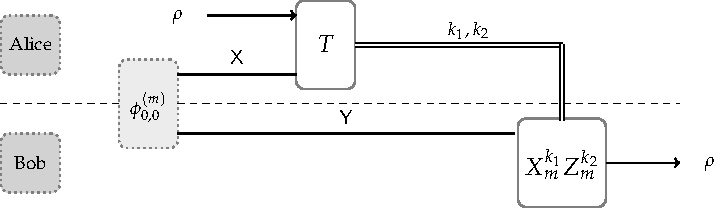
\includegraphics[scale=1.0]{figures/teleportation.pdf}
	\end{center}
		\caption[The teleportation protocol.]{The teleportation protocol. Alice's goal is to teleport the state $\rho$ to Bob. The dashed line in the center separates the actions of Alice and Bob. Alice and Bob prepare a maximally entangled state where part of the state is contained in Alice's register $\reg{X}$ and the other part is contained in Bob's register $\reg{Y}$. Alice performs a Bell measurement and sends $k_1,k_2 \in \integer_m$, from this measurement to Bob. Bob receives $k_1$ and $k_2$ and applies of the generalized Pauli operators to his register $\reg{Y}$. The end result is that Bob now possesses the state $\rho$. }
	\label{fig:teleportation}
\end{figure}

Suppose that Alice and Bob prepare registers $(\reg{X},\reg{Y})$ where Alice holds $\reg{X}$ and Bob holds $\reg{Y}$ such that 
\begin{align}
	\abs{\reg{X}} = m = \abs{\reg{Y}},
\end{align}
where the contents of $(\reg{X},\reg{Y})$ corresponds to the maximally entangled state $\phi_{0,0}^{(m)}$. Alice obtains a new state, $\rho$, contained in register $\reg{Z}$ that she desires to send to Bob. In order to do so, both parties abide by the generalized teleportation protocol, that is depicted in Figure~\ref{fig:teleportation}.

\begin{enumerate}
\item Alice measures $(\reg{Z},\reg{X})$ with respect to the generalized Bell basis as defined from equation~\eqref{eq:generalized-bell-basis}
\begin{align}
	\left \{ \phi^{(m)}_{k_1, k_2} : k_1, k_2 \in \integer_m \right \},
\end{align}
where the outcomes of performing this measurement are given by $(k_1,k_2) \in \integer_{m} \times \integer_{m}$. 

\item Alice then sends measurement outcomes $(k_1,k_2)$ to Bob.

\item Bob receives $(k_1,k_2)$ from Alice and applies the generalized Pauli operator 
	\begin{align}
		W_{k_1,k_2}^{(m)},
	\end{align}
as defined in equation~\eqref{eq:generalized-pauli-ops} to his register, $\reg{Y}$, which completes the protocol, and teleports $\reg{Z}$ to Bob. 
\end{enumerate}
To see why the state $\rho$ from Alice is teleported to Bob, one may consider a generalization of the case for $m = 2$. The scenario where $m = 2$ is the most standard teleportation setup, and has been covered, for instance, in~\cite{Nielsen2001}, whereas the generalization is covered in~\cite{Wilde2013}.

%To see why the register $\reg{Z}$ from Alice is teleported to Bob, consider the case of $m = 2$. Alice and Bob prepare a maximally entangled state in their registers $(\reg{X},\reg{Y})$ as 
%\begin{align}
%	u = \frac{1}{\sqrt{2}} \left( e_0 \otimes e_0 + e_1 \otimes e_1 \right).
%\end{align}
%Since $m = 2$, we assume that Alice's register $\reg{Z}$ contains a qubit pure state $v \in \complex^{\Sigma}$ with $\Sigma = \{0,1\}$ that Alice intends to teleport to Bob. We may write the vector $v$ as
%\begin{align}
%	v = \alpha e_0 + \beta e_1
%\end{align}
%for some $\alpha,\beta \in \complex$ such that $\abs{\alpha}^2 + \abs{\beta}^2 = 1$. The contents of Alice's registers $(\reg{Z},\reg{X})$ may be written as 
%\begin{equation} \label{eq:telep-alice-state}
%	\begin{aligned}
%		v \otimes u &= \left( \alpha e_0 + \beta e_1 \right) \otimes \left( \frac{1}{\sqrt{2}} \left( e_0 \otimes e_0 + e_1 \otimes e_1 \right) \right) \\
%		&= \frac{1}{\sqrt{2}} \left( \alpha \left( e_0 \otimes e_0 \otimes e_0 \right) + \beta \left( e_1 \otimes e_0 \otimes e_0 \right) + \alpha \left( e_0 \otimes e_1 \otimes e_1 \right) + \beta \left( e_1 \otimes e_1 \otimes e_1 \right) \right).
%	\end{aligned}
%\end{equation}
%It will be useful to us if we can write equation~\eqref{eq:telep-alice-state} in terms of the Bell states. Indeed, by using the following fact that
%\begin{equation}
%	\begin{aligned}
%		e_0 \otimes e_0 = \frac{1}{\sqrt{2}} \left( \phi_{0} + \phi_{3} \right), &\quad e_0 \otimes e_1 = \frac{1}{\sqrt{2}} \left( \phi_{1} + \phi_{2} \right) \\
%		e_1 \otimes e_0 = \frac{1}{\sqrt{2}} \left( \phi_{1} - \phi_{2} \right) &\quad e_1 \otimes e_1 = \frac{1}{\sqrt{2}} \left( \phi_{0} - \phi_{3} \right),
%	\end{aligned}
%\end{equation}
%we can perform some algebraic manipulation to write equation~\eqref{eq:telep-alice-state} as 
%\begin{equation} \label{eq:telep-alice-state-2}
%	\begin{aligned}
%		&\frac{1}{2} \left( \alpha \left( \phi_{0} + \phi_{3} \right) \otimes e_0 + \beta \left( \phi_{1} + \phi_{2} \right)\otimes e_0 + \alpha \left( \phi_{1} - \phi_{2} \right) \otimes e_1 + \beta \left( \phi_{0} - \phi_{3} \right) \otimes e_1 \right) \\
%		&= \frac{1}{2} \left( \phi_{0} \otimes \left( \alpha e_0 + \beta e_1 \right) + \phi_{2} \otimes \left( \alpha e_0 - \beta e_1 \right) + \phi_{1} \otimes \left( \alpha e_1 + \beta e_0 \right) + \phi_{2} \otimes \left(\alpha e_1 - \beta e_0 \right) \right).
%	\end{aligned}
%\end{equation}
%We note that equation~\eqref{eq:telep-alice-state-2} may be written in terms of the Pauli-$X$ and Pauli-$Z$ operators. Further simplifications allow us to write the equation in terms of the generalized Bell states and generalized Pauli operators for $m = 2$ where
%\begin{equation} \label{eq:telep-alice-state-3}
%	\begin{aligned}
%		&= \frac{1}{2} \left( \phi_{0} \otimes v + \phi_{3} \otimes Z v + \phi_{1} \otimes X v + \phi_{2} \otimes XZ v \right).
%	\end{aligned}
%\end{equation}
%In the first step of the teleportation protocol, Alice performs a measurement on $(\reg{Z},\reg{X})$ in the Bell basis. Alice then has an equal chance of obtaining any of the four states
%\begin{align}
%	\phi_{0} \otimes v, \quad \phi_{3} \otimes Z v, \quad \phi_{1} \otimes X v, \quad \textnormal{or} \quad \phi_{2} \otimes X Z v.
%\end{align}
%Since Alice knows the result of the measurement, she knows if Bob's state is either $v$, $Zv$, $Xv$, or $XZv$. Alice sends $m = 2$ bits of communication to Bob to indicate which of the four measurement outcomes she received. When Bob receives this information, he is now aware of what Pauli operators to apply to his register, $\reg{Y}$. The act of Bob applying the appropriate Pauli operators to his register teleports the contents of the register $\reg{Z}$ to Bob. 


%-------------------------------------------------------------------------------
\section{The nonlocal game model}
\label{sec:the-nonlocal-games-model}
%-------------------------------------------------------------------------------

%The model of nonlocal games arose from the fields of theoretical physics and classical complexity theory. In terms of theoretical physics, the underpinnings of this model were first arguably laid down in the seminal paper by Einstein, Podolsky, and Rosen~\cite{Einstein1935}. In this work, the authors considered a thought experiment that sought to illustrate the incompleteness of quantum theory. The notion of entanglement itself was particularly unsettling to the authors, as it would appear that the behavior of entangled particles leads one to postulate on the existence of so-called ``hidden variables''; some inherent property in such a system that is hidden to us as observers of the system. In 1964, the physicist John Bell followed up on the work of~\cite{Einstein1935} and developed a theorem to test for the existence of hidden variables. John Bell proposed an inequality that illustrated the inability of a local hidden variable theory to account for certain consequences of entanglement.

%\comment{some stuff here on Bell inequalities and nonlocal games} 

%\comment{Mention nonlocal games == bell inequalities}.

%While the historical and physical aspects of the beginnings of nonlocal games are intriguing, in this thesis, we shall primarily view the nonlocal games model through the lens of computer science. Indeed, the nonlocal games model is in equal parts built upon the notion of \emph{interactive proof systems}, as initially introduced in~\cite{Goldwasser1985} and independently in~\cite{Babai1985}, and further studied in classical complexity theory~\cite{Ben-Or1988,Fortnow1989,Babai1991,Feige1991,Feige1994,Raz1998}. Informally, an interactive proof system is an abstract model of computation where two parties, referred to as the ``prover'' and the ``verifier'', exchange messages to determine the validity of mathematical statement. The interactive proof system model was made more powerful in~\cite{Ben-Or1988}, where the authors introduced a multi-prover interactive proof system that consisted of two independent provers. These two provers, which we refer to as Alice and Bob respectively, are unable to communicate once the protocol begins. In~\cite{Cleve2004}, the authors formally introduced a multi-prover interactive proof system where the provers and verifier may exchange and process quantum information. Such a model is referred to as a \emph{nonlocal game}. These two independent lines of research on nonlocal games from the sides of physics and computer science have since been merged in the context of quantum information and computation, and the result has been an active topic of research~\cite{Cleve2004, Brassard2005, Cleve2008, Doherty2008,Kempe2010,Kempe2010a,Kempe2011,Junge2011a,Buhrman2013,
%Regev2013,Dinur2013,Vidick2013,Cleve2014}.

The nonlocal game model is built upon the notion of \index{interactive proof system}{\emph{interactive proof systems}}, initially introduced in~\cite{Goldwasser1985} and independently in~\cite{Babai1985}, and further studied in classical complexity theory~\cite{Ben-Or1988,Fortnow1989,Babai1991,Feige1991,Feige1994,Raz1998}. Informally, an interactive proof system is an abstract model of computation where two parties, referred to as the \index{prover (interactive proof system)}{\emph{prover}} and the \index{verifier (interactive proof system)}{\emph{verifier}}, exchange messages to determine the validity of a mathematical statement. The interactive proof system model was made more powerful in~\cite{Ben-Or1988}, where the authors introduced a multi-prover interactive proof system that consisted of at least two independent provers, and one verifier. When considering two provers, we refer to them by the names of \emph{Alice} and \emph{Bob}, and we call the verifier the \emph{referee}. We refer to a one-round multi-prover interactive proof system with at least two provers (Alice and Bob) that play cooperatively against a referee as a \index{nonlocal game}{\emph{nonlocal game}}. In~\cite{Cleve2004}, the authors formally introduced the notion of a nonlocal game where the provers may share entanglement. The nonlocal game model served to embody the notion of a \index{Bell inequality}{\emph{Bell inequality}}, an inequality that illustrated the inability of a local hidden variable theory to account for certain consequences of entanglement~\cite{Bell1964}. In~\cite{Clauser1969}, the authors Clauser, Horne, Shimony, and Holt presented a special type of Bell inequality that has since been named after the authors as the \index{CHSH inequality}{\emph{CHSH inequality}}. In~\cite{Cleve2004}, the CHSH inequality was first formulated in the language of nonlocal games. Nonlocal games have since been studied in the context of quantum information, and the result has been an active topic of research~\cite{Cleve2004, Brassard2005, Cleve2008, Doherty2008,Kempe2010,Kempe2010a,Kempe2011,Junge2011a,Buhrman2013,
Regev2013,Dinur2013,Vidick2013,Cleve2014}.



More formally, a nonlocal game begins by the referee selecting a pair of questions $(x,y)$ according to a fixed probability distribution that is known to all parties. The referee then sends question $x$ to Alice and question $y$ to Bob. While we assume that Alice and Bob may confer prior to the start of the game, when the game begins, the players are forbidden from communicating with each other. So Alice is unaware of the question that Bob received, and vice versa. Alice and Bob then respond to the referee with answers $a$ and $b$, respectively. Upon receiving these answers, the referee evaluates some predicate based on the questions and answers to determine whether Alice and Bob win or lose. In addition to having complete knowledge of the probability distribution used to select $x$ and $y$, we also assume that Alice and Bob have complete knowledge of the predicate.

The goal of Alice and Bob is to maximize their probability of obtaining a winning outcome. Prior to the start of the game, Alice and Bob may corroborate on a joint \index{strategy}{\emph{strategy}} to achieve this goal. One may consider a number of strategies for nonlocal games. For example, if Alice and Bob make use of classical resources, we call this a \emph{classical strategy}. In such a strategy, the players answer \emph{deterministically} with answers $a$ and $b$ determined by functions of $x$ and $y$ respectively. The players may also make use of randomness, but doing so provides no advantage over simply playing deterministically. 

Another type of strategy that the players may adopt are \emph{quantum strategies}. In a quantum strategy, Alice and Bob prepare and share a joint quantum system prior to the start of the game. We also assume that the players have local sets of measurement operators that they perform on their share of the state after the game has begun and they have received their questions from the referee to determine their answers $a$ and $b$. 

One may consider a number of sub-classifications of quantum strategies as well. For instance, the size of the shared quantum system may make a difference in how well Alice and Bob can perform, and indeed one can ask whether or not the size of the state yields any advantage. Another sub-classification of a quantum strategy is referred to as a \emph{commuting measurement strategy}. In this type of strategy, the bipartite tensor product structure of a shared quantum system between Alice and Bob is relaxed to one in which the local measurements of Alice and Bob pairwise commute. 

An even more general type of strategy that Alice and Bob may adopt is referred to as a \emph{non-signaling strategy}. In this type of strategy, the only constraint on Alice and Bob is that they cannot communicate during the game, but may make use of any type of resource, even possibly those outside of the scope of resources described by quantum mechanics. 

We refer to the \index{value (nonlocal game)}{\emph{value}} of a nonlocal game as the supremum value of the probability for the players to win over all strategies of a specified type. 

%-------------------------------------------------------------------------------
\subsection{Strategies for nonlocal games}
\label{sec:strategies-for-nonlocal-games}
%-------------------------------------------------------------------------------

%-------------------------------------------------------------------------------
\subsubsection*{Nonlocal games and correlation functions}
\label{sec:correlation-operators-for-nonlocal-games}
%-------------------------------------------------------------------------------

We specify a nonlocal game, $G$, as a pair $(\pi,V)$ where $\pi$ is a probability distribution of the form 
\begin{align}
	\pi : \SigmaA \times \SigmaB \rightarrow \left[0,1\right]
\end{align}
on the Cartesian product of two alphabets $\SigmaA$ and $\SigmaB$, and $V$ is a function of the form 
\begin{align}
	V : \GammaA \times \GammaB \times \SigmaA \times \SigmaB \rightarrow \left[0,1\right],
\end{align}
for $\SigmaA$ and $\SigmaB$ as above and $\GammaA$ and $\GammaB$ being alphabets. We use
\begin{align}
	\Sigma = \SigmaA \times \SigmaB \quad \textnormal{and} \quad \Gamma = \GammaA \times \GammaB
\end{align}
to denote the respective sets of questions asked to Alice and Bob and the sets of answers sent from Alice and Bob to the referee. 

For any type of strategy, the output probability distributions produced by Alice and Bob may be described by a function
\begin{align}
	C : \GammaA \times \GammaB \times \SigmaA \times \SigmaB \rightarrow [0,1],
\end{align}
where the function $C$ is referred to as a \index{correlation function (nonlocal game)}{\emph{correlation function}}. The entry $C(a,b|x,y)$ corresponds to the probability that Alice and Bob output $a \in \GammaA$ and $b \in \GammaB$ given the input $x \in \SigmaA$ and $y \in \SigmaB$. Since a correlation function represents a collection of probability distributions, the operator $C$ must satisfy 
\begin{align}
	\sum_{(a,b) \in \Gamma} C(a,b|x,y) = 1
\end{align}
for all $x \in \SigmaA$ and $y \in \SigmaB$. In particular, Alice and Bob's winning probability is represented as 
\begin{align} \label{eq:correlation-function}
	\sum_{(x,y) \in \Sigma} \pi(x,y) \sum_{(a,b) \in \Gamma} V(a,b|x,y) C(a,b|x,y),
\end{align}
where the correlation function is defined with respect to the corresponding strategy implemented by Alice and Bob. 

In the coming sections, we shall make the notions of the value of a nonlocal game and their corresponding strategies more concrete. 

%-------------------------------------------------------------------------------
\subsubsection*{Quantum strategies for nonlocal games}
\label{sec:quantum-strategies-for-nonlocal-games}
%-------------------------------------------------------------------------------

A \index{quantum strategy (nonlocal game)}{\emph{quantum strategy}} for a nonlocal game consists of complex Euclidean spaces $\U$ for Alice and $\V$ for Bob, a quantum state $\sigma \in \Density(\U \otimes \V)$ contained in registers $(\reg{U},\reg{V})$, and two collections of measurements, 
\begin{align}
	\{ A_a^x : a \in \GammaA \} \subset \Pos(\U) \quad \textnormal{and} \quad \{ B_b^y : b \in \GammaB \} \subset \Pos(\V), 
\end{align}
for each $x \in \SigmaA$ and $y \in \SigmaB$ respectively. The measurement operators satisfy the constraint that 
\begin{align}
	\sum_{a \in \GammaA} A_a^x = \I_{\U} \quad \textnormal{and} \quad \sum_{b \in \GammaB} B_b^y = \I_{\V}
\end{align}
for each $x \in \SigmaA$ and $y \in \SigmaB$. 

At the beginning of the game, Alice and Bob prepare a quantum system represented by the bipartite state $\sigma \in \Density(\U \otimes \V)$. The referee then selects questions $(x,y) \in \Sigma$ according to the probability distribution $\pi$ that is known to Alice, Bob, and the referee. The referee then sends $x$ to Alice and $y$ to Bob. Alice and Bob then generate answers $a \in \GammaA$ and $b \in \GammaB$, by making measurements on their portion of the state $\sigma$. That is to say, Alice makes a measurement on her part of $\sigma$ with respect to the measurement operators $\{ A_a^x : a \in \GammaA \}$. Similarly, Bob also performs a measurement on his part of $\sigma$ using the set of measurement operators $\{ B_b^y : b \in \GammaB \}$. The answers $(a,b)$ are then sent to the referee. The referee now possesses the questions $(x,y)$ in addition to the responses sent by Alice and Bob, $(a,b)$. The referee uses this information to evaluate the predicate $V(a,b|x,y)$, resulting in either a winning or losing outcome, represented by a $1$ or a $0$, respectively. A depiction of a nonlocal game is given in Figure~\ref{fig:nonlocal-game}. 

\begin{figure}[!htpb] 
	\begin{center}
		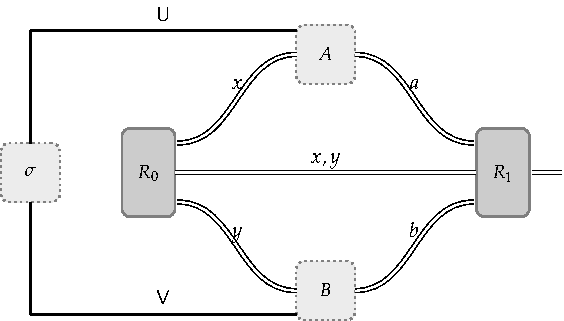
\includegraphics[scale=1.0]{figures/nonlocal_game.pdf}
	\end{center}
		\caption[A two-player nonlocal game.]{A two-player nonlocal game. In a nonlocal game, the players, Alice and Bob, first select a strategy. In the case of a quantum strategy, Alice and Bob may share a state $\sigma \in \Density(\U \otimes \V)$ in registers $(\reg{U},\reg{V})$. We assume that after this point, Alice and Bob are space-like separated and unable to communicate with each other for the remainder of the game. The referee then selects and sends questions $x \in \SigmaA$ for Alice and $y \in \SigmaB$ for Bob according to the publicly known probability distribution, $\pi$. The referee also keeps a copy of $x$ and $y$ after sending. Alice and Bob generate their answers $a \in \GammaA$ and $b \in \GammaB$ respectively, and send their answers to the referee, where the predicate $V(a,b|x,y)$ is computed to determine the probability that Alice and Bob win or lose.}
\label{fig:nonlocal-game}
\end{figure}

The winning probability for such a strategy in this game $G = (\pi,V)$ is given by equation~\eqref{eq:correlation-function} where $C$ is a \index{quantum correlation function (nonlocal game)}{\emph{quantum correlation function}} defined as 
\begin{align}
		C(a,b|x,y) = \bigip{A_a^x \otimes B_b^y}{\sigma},
\end{align}
for all $x \in \SigmaA$, $y \in \SigmaB$, $a \in \GammaA$, and $b \in \GammaB$. 

The \index{quantum value (nonlocal game)}{\emph{quantum value}} of a nonlocal game $G$, denoted as $\omega^*(G)$, is the supremum value of the winning probability of $G$ taken over all quantum strategies for Alice and Bob. We may also write $\omega_N^*(G)$ to denote the quantum value of $G$ when the dimension of Alice's space and the dimension of Bob's space is equal to $N$. Note that we can make the assumption on Alice and Bob's spaces that
\begin{align}
	\dim(\A) = \dim(\B),
\end{align} 
since whichever strategy Alice and Bob use, the probability of winning is always going to be maximized when $\sigma$ is a pure state. That is, Alice and Bob will not perform any better for any possible convex combination of $\sigma$, so we may as well assume $\sigma$ to be pure, that is $\sigma = uu^*$ for some nonzero vector $u \in \U \otimes \V$. It holds that one can always take the Schmidt decomposition of $u$, where it can be observed that the state is supported on spaces of equal dimension. 

We use $\Q_N(\GammaA, \GammaB | \SigmaA, \SigmaB)$ to denote the set of all quantum correlation functions when the dimension of Alice and Bob's system is equal to $N$. 


%-------------------------------------------------------------------------------
\subsubsection*{Classical strategies for nonlocal games}
\label{sec:classical-strategies-for-nonlocal-games}
%-------------------------------------------------------------------------------

A \index{classical strategy (nonlocal game)}{\emph{classical strategy}} for a nonlocal game consists of functions $f : \SigmaA \rightarrow \GammaA$ and $g : \SigmaB \rightarrow \GammaB$ that deterministically produce an output for every input. This type of classical strategy is referred to as a \index{deterministic strategy}{\emph{deterministic strategy}}, as the outputs are produced deterministically. Provided that we are interested in maximizing the winning probability, there is no loss in generality in restricting our attention to deterministic strategies for any classical strategy, as the classical value of any nonlocal game will always be obtained by such a deterministic strategy. This can be observed by the fact that any probabilistic strategy may be expressed as a convex combination of deterministic strategies, so Alice and Bob gain no benefit from using randomness. In other words, the average is never bigger than the maximum. The winning probability for such a strategy in this game $G = (\pi,V)$ is given by
\begin{align}
	\sum_{(x,y) \in \Sigma} \pi(x,y) \sum_{(a,b) \in \Gamma} V(a,b|x,y) C(a,b|x,y),
\end{align}
where $C$ is the \index{deterministic correlation function (nonlocal game)}{\emph{deterministic correlation function}} defined as 
\[
 C(a,b|x,y) =
  \begin{cases} 
      \hfill 1 \hfill & \text{ if $a = f(x) \textnormal{ and } b = g(y)$,} \\
      \hfill 0 \hfill & \text{ otherwise,} \\
  \end{cases}
\]
for all $x \in \SigmaA$, $y \in \SigmaB$, $a \in \GammaA$, and $b \in \GammaB$. We use $\L(\GammaA,\GammaB|\SigmaA,\SigmaB)$ to denote the set of all deterministic correlation functions, including all convex combinations of deterministic correlation functions as well.

The \index{classical value (nonlocal game)}{\emph{classical value}} of a nonlocal game $G$, denoted as $\omega(G)$ is the supremum value of the winning probability of $G$ taken over all classical strategies for Alice and Bob. As argued above the supremum value is necessarily achieved by some deterministic strategy, and therefore we may write $\omega(G)$ as 
\begin{align}
	\omega(G) = \max_{f,g} \sum_{(x,y) \in \Sigma} \pi(x,y) V(f(x),g(y)|x,y),
\end{align}
where the maximum is over all functions $f: \SigmaA \rightarrow \GammaA$ and $g: \SigmaB \rightarrow \GammaB$. 

%-------------------------------------------------------------------------------
\subsubsection*{Commuting measurement strategies for nonlocal games}
\label{sec:commuting-measurement-strategies-for-nonlocal-games}
%-------------------------------------------------------------------------------

A \index{commuting measurement strategy (nonlocal game)}{\emph{commuting measurement strategy}} consists of a single (possibly infinite-dimensional) Hilbert space, $\H$, a quantum state $\sigma \in \Density(\H)$, and two collections of measurements, 
\begin{align}
	\{ A_a^x : a \in \GammaA \} \subset \Pos(\H) \quad \textnormal{and} \quad \{ B_b^y : b \in \GammaB \} \subset \Pos(\H),
\end{align}
such that 
\begin{align}
	\sum_{a \in \GammaA} A_a^x = \sum_{b \in \GammaB} B_b^y = \I_{\H}
\end{align}
for all $x \in \SigmaA$ and $y \in \SigmaB$, and that satisfy
\begin{align}
	\left[ A_a^x, B_b^y \right] = 0
\end{align}
for all $x \in \SigmaA, y \in \SigmaB, a \in \GammaA,$ and $b \in \GammaB$. For a nonlocal game, $G = (\pi,V)$, the winning probability for a commuting measurement strategy is given by equation~\eqref{eq:correlation-function} where $C$ is a \index{commuting measurement correlation function (nonlocal game)}{\emph{commuting measurement correlation function}} defined as 
\begin{align}
	C(a,b|x,y) = \bigip{A_a^x B_b^y}{\sigma}
\end{align}
for all $x \in \SigmaA$, $y \in \SigmaB$, $a \in \GammaA$, and $b \in \GammaB$. We use $\C(\GammaA, \GammaB | \SigmaA, \SigmaB)$ to denote the set of all commuting measurement correlation function. 

The \index{commuting measurement value (nonlocal game)}{\emph{commuting measurement value}} of a nonlocal game $G$, denoted as $\omega_c(G)$, is the supremum value of the winning probability of $G$ taken over all commuting measurement strategies for Alice and Bob. Elsewhere in the literature, the commuting measurement value is also referred to as the field-theoretic value~\cite{Doherty2008}. 

%-------------------------------------------------------------------------------
\subsubsection*{Non-signaling strategies for nonlocal games}
\label{sec:non-signaling-strategies-for-nonlocal-games}
%-------------------------------------------------------------------------------

For a nonlocal game $G = (\pi,V)$, the winning probability for a \index{non-signaling strategy}{\emph{non-signaling strategy}} is given by equation~\eqref{eq:correlation-function} where $C$ is a \index{non-signaling correlation function (nonlocal game)}{\emph{non-signaling correlation function}} that satisfies the following non-signaling properties
\begin{align} \label{eq:ns-constraints-1}
	\sum_{b \in \GammaB} C(a,b|x,y) = \sum_{b \in \GammaB} C(a,b|x,y^{\prime}),
\end{align}
for all $a \in \GammaA$, $x \in \SigmaA$, $y \in \SigmaB$, and $y^{\prime} \in \SigmaB$ and 
\begin{align} \label{eq:ns-constraints-2}
	\sum_{a \in \GammaA} C(a,b|x,y) = \sum_{a \in \GammaA} C(a,b|x^{\prime},y),
\end{align}
for all $b \in \GammaB$, $x \in \SigmaA$, $x^{\prime} \in \SigmaA$, and $y \in \SigmaB$ and where $C$ is normalized and nonnegative. We use $\NS(\GammaA, \GammaB | \SigmaA, \SigmaB)$ to denote the set of all non-signaling correlation functions. 

The \index{non-signaling value (nonlocal game)}{\emph{non-signaling value}} of a nonlocal game, $G$, denoted as $\omega_{\ns}(G)$, is the supremum value of the winning probability of $G$ taken over all non-signaling strategies for Alice and Bob.

If one wishes, one may even consider a more general type of strategy, indeed the most general strategy one may consider in the realm of nonlocal games. This most general type of strategy, referred to as a \index{global strategy}{\emph{global strategy}} is one in which the correlation functions need only satisfy
\begin{align}
	\sum_{(a,b) \in \Gamma} C(a,b|x,y) = 1, 
\end{align}
for all $x \in \SigmaA$ and $y \in \SigmaB$ and that the entries of $C$ be nonnegative. Indeed, these two constraints are in all of the strategies we have considered thus far, as they are implicit from the definition of a correlation function from Section~\ref{sec:correlation-operators-for-nonlocal-games}. Another way to think about non-signaling strategies therefore is to consider them as strategies that satisfy these two implicit restrictions of a global strategy, as well as the non-signaling constraints from equations~\eqref{eq:ns-constraints-1}~and~\eqref{eq:ns-constraints-2}.  

%% Refer to page 37 of Quantum Information, Bell Inequalities and the No-Signalling Principle and Jamie's slides
%A \index{non-signaling strategy (nonlocal game)}{\emph{non-signaling strategy}} consists of finite-dimensional complex Euclidean spaces $\A$ for Alice and $\B$ for Bob, a quantum states $\sigma \in \Density(\A \otimes \B)$, and two collections of measurements 
%\begin{align}
%	\{ A^x_a : a \in \GammaA \} \subset \Pos(\A) \quad \textnormal{and} \quad \{ B^y_b : b \in \GammaB \} \subset \Pos(\B),
%\end{align}
%for each $x \in \SigmaA$ and $y \in \SigmaB$ respectively that satisfy the following constraints
%\begin{equation} \label{eq:ns-alice-marginals}
%	\begin{aligned}
%		\sum_{b \in \GammaB} \biggip{A_a^x \otimes B_b^y}{A_a^x \otimes B_b^y \sigma} = \sum_{b \in \GammaB} \biggip{A_a^x \otimes B_b^{y^{\prime}}}{A_a^x \otimes B_b^{y^{\prime}} \sigma},
%	\end{aligned}
%\end{equation}
%for all $a \in \GammaA$ and $(x,y,y^{\prime}) \in \SigmaA \times \SigmaB$ where $y \not= y^{\prime}$ and 
%\begin{equation} \label{eq:ns-bob-marginals}
%	\begin{aligned}
%		\sum_{a \in \GammaA} \biggip{A_a^x \otimes B_b^y}{A_a^x \otimes B_b^y \sigma} = \sum_{a \in \GammaA} \biggip{A_a^{x^{\prime}} \otimes B_b^y}{A_a^{x^{\prime}} \otimes B_b^y \sigma},
%	\end{aligned}
%\end{equation}
%for all $b \in \GammaB$ and $(x,x^{\prime},y) \in \SigmaA \times \SigmaB$ where $x \not= x^{\prime}$. 
%
%For a nonlocal game $G = (\pi,V)$, the expected payoff for a non-signaling strategy is given by
%\begin{align}
%	\sum_{(x,y) \in \SigmaA \times \SigmaB} \pi(x,y) \sum_{(a,b) \in \GammaA \times \GammaB} V(a,b|x,y) C((x,a),(y,b)), 
%\end{align}
%where the operator $C$ is a \index{non-signaling correlation operator (nonlocal game)}{\emph{non-signaling correlation operator}} if it satisfies the constraints from equations~\eqref{eq:ns-alice-marginals} and~\eqref{eq:ns-bob-marginals} for all $x \in \SigmaA$, $y \in \SigmaB$, $a \in \GammaA$, and $b \in \GammaB$. We use $\NS$ to denote the set of all non-signaling correlation operators. The \index{non-signaling value (nonlocal game)}{\emph{non-signaling value}} of a nonlocal game $G$, denoted as $\omega_{\ns}(G)$, is the supremum value of the expected payoff of $G$ taken over all non-signaling measurement strategies for Alice and Bob.  
%
%Non-signaling strategies are aptly named as they represent the fact that the information of Bob's question, $y \in \SigmaB$, cannot influence the measurement operator that Alice applies, $A_a^x$, as this information transfer is limited by the speed of light. In other words, Bob cannot ``signal'' his question to Alice without violating special relativity, and similarly, Alice cannot ``signal'' her question to Bob for the same reason. Expressing this in a more mathematical way, we say that the probability of Alice's actions are independent of the question sent to Bob, and vice versa. Specifically, equation~\eqref{eq:ns-alice-marginals} is equivalent to
%\begin{align}
%\bigip{A_a^x}{A_a^x \tr_{\B}(\sigma)},
%\end{align}
%and similarly, equation~\eqref{eq:ns-bob-marginals} is equivalent to 
%\begin{align}
%\bigip{B_b^y}{B_b^y \tr_{\A}(\sigma)}.
%\end{align}

%-------------------------------------------------------------------------------
\subsection{Relationships between different strategies and values} \label{sec:relationships-between-different-strategies-and-values}
%-------------------------------------------------------------------------------

%\comment{perhaps here place a proof of the fact that the classical and NS sets of polytopes / convex? and that quantum isn't}

In order to determine how well the players can expect to do for a particular choice of strategy, we consider the corresponding values for each strategy. There exist algorithms that allow one to calculate the classical and non-signaling values of an arbitrary nonlocal game by optimizing over the respective classical and non-signaling correlation functions~\cite{Brunner2014}. These algorithms are not particularly efficient however, as there are exponentially many possible functions for Alice and Bob to consider. In general, with the exception of a specific class of nonlocal games~\cite{Cleve2008}, there is no known efficient algorithm to exactly compute the quantum value of an arbitrary nonlocal game. There is, however, an approach that allows one to approximate the quantum values of arbitrary nonlocal games~\cite{Doherty2008,Navascues2007,Navascues2008}, a technique we will investigate in greater detail in Chapter~\ref{chap:extended_npa_hierarchy}.  

The sets of correlation functions for the strategies we have covered thus far have the following relationship 
\begin{align}
	\L(\GammaA, \GammaB | \SigmaA, \SigmaB) \subseteq \Q(\GammaA, \GammaB | \SigmaA, \SigmaB) \subseteq \C(\GammaA, \GammaB | \SigmaA, \SigmaB) \subseteq \NS(\GammaA, \GammaB | \SigmaA, \SigmaB),
\end{align}
for alphabets $\GammaA, \GammaB, \SigmaA$ and $\SigmaB$. The relationship of $\L(\GammaA, \GammaB | \SigmaA, \SigmaB) \subseteq \Q(\GammaA, \GammaB | \SigmaA, \SigmaB)$ follows since Alice and Bob could use their shared entangled state only as a source of shared randomness. Recall, that Alice and Bob gain no benefit from using randomness in a classical strategy, so one may restrict attention to classical strategies defined in terms of deterministic ones. Should Alice and Bob use their quantum state in a quantum strategy as a source of shared randomness, this is no better than having them use a classical strategy, and gives the relationship between correlation functions. The relationship that $\Q(\GammaA, \GammaB | \SigmaA, \SigmaB) \subseteq \C(\GammaA, \GammaB | \SigmaA, \SigmaB)$ holds due to the fact that bipartite operators where the identity operator is on either side of the operator obey the commutation relationship, that is
\begin{align}
	\left[ A_a^x \otimes \I_{\B}, \I_{\A} \otimes B_b^y \right] = 0
\end{align}
for sets of operators $\{A_a^x : a \in \GammaA\}$ and $\{B_b^y : b \in \GammaB\}$ over all $x \in \SigmaA$, $y \in \SigmaB$, $a \in \GammaA$, and $b \in \GammaB$. The relationship that $\Q(\GammaA, \GammaB | \SigmaA, \SigmaB) \subseteq \NS(\GammaA, \GammaB | \SigmaA, \SigmaB)$ comes from observing that for a commuting measurement correlation function
\begin{align}
	C(a,b|x,y) = \bigip{A_a^x B_b^y}{\sigma}
\end{align}
we have that
\begin{align}
	\sum_{b \in \GammaB} C(a,b|x,y) = \sum_{b \in \GammaB} \bigip{A_a^x B_b^y}{\sigma} = \bigip{A_a^x}{\sigma},
\end{align}
or in other words, that there is no dependence on $y$. Similarly, we have that
\begin{align}
	\sum_{a \in \GammaA} C(a,b|x,y) = \sum_{a \in \GammaA} \bigip{A_a^x B_b^y}{\sigma} = \bigip{B_b^y}{\sigma}.
\end{align}

% the fact that any quantum correlation operator satisfies the non-signaling conditions, however there do exist quantum correlation operators that do not satisfy the constraints of a classical correlation operator. These are in fact examples of Bell inequality violations, or nonlocal games that exhibit a higher quantum value than classical value. It also holds that there exist non-signaling correlation operators that do not obey the constraints of a quantum correlation operator~\cite{Khalfin1985,Rastall1985,Popescu1994}. The relationship that $\C(\Sigma,\Gamma) \subset \NS(\Sigma,\Gamma)$ follows a similar line of reasoning. 

Given that the correlation functions obey these relationships, it then follows that the corresponding values of these operators must also satisfy a similar inequality relationship
\begin{align}
	0 \leq \omega(G) \leq \omega^*(G) \leq \omega_c(G) \leq \omega_{\ns}(G) \leq 1. 
\end{align}

%\comment{How all the values relate to one another}

%\comment{Mention the difficulty of computing the quantum value, etc.}

%It is known that quantum strategies will perform no better than commuting measurement strategies in the case where the measurement operators of Alice and Bob are finite dimensional~\cite{Tsirelson1993,Doherty2008,Navascues2012}. In other words, for alphabets $\Sigma$ and $\Gamma$, the set of quantum correlation operators, $\Q_n(\Sigma,\Gamma)$, and the set commuting correlation operators, $\C_n(\Sigma,\Gamma)$, has the property that $\Q_n(\Sigma,\Gamma) = \C_n(\Sigma,\Gamma)$ when $n$ is finite. A long-standing open question of Tsirelson~\cite{Tsirelson2006}, referred to as the \index{strong Tsirelson conjecture}{\emph{strong Tsirelson conjecture}}~\cite{Dykema2016}, asks whether this is also true in the case where the measurement operators are infinite dimensional. In the infinite-dimensional case, it does hold that $\Q_n(\Sigma,\Gamma) \subseteq \C_n(\Sigma,\Gamma)$ since 
%\begin{align}
%	\left[A_a^x \otimes \I_{\B}, \I_{\A} \otimes B_b^y \right] = 0,
%\end{align}
%however showing the reverse implication has proven to be a difficult problem. Recently, a result of Slofstra~\cite{Slofstra2016} proved that the equality for these two sets does not hold in the infinite-dimensional case, that is, $\Q_n(\Sigma,\Gamma) \not= \C_n(\Sigma,\Gamma)$, which negatively resolved the strong Tsirelson conjecture.  
%
%For alphabets $\Sigma$ and $\Gamma$, we may consider the following sets of correlation operators $\Q_{n \rightarrow \infty}(\Sigma,\Gamma)$ and $\C_{n \rightarrow \infty}(\Sigma,\Gamma)$ that consist of all games, $G$ such that 
%\begin{align}
%	\lim_{n \rightarrow \infty} \omega_n^*(G) = 1 \quad \textnormal{and} \quad \lim_{n \rightarrow \infty} \omega_c(G) = 1,
%\end{align}
%where $n$ corresponds to the dimension of the state held by Alice and Bob, respectively. The \index{weak Tsirelson conjecture}{\emph{weak Tsirelson conjecture}} concerns itself with these sets and asks whether or not $\Q_{n \rightarrow \infty}(\Sigma,\Gamma) = \C(\Sigma,\Gamma)$, or equivalently, whether $\C_{n \rightarrow \infty}(\Sigma,\Gamma) = \C(\Sigma,\Gamma)$. This question remains open, and furthermore, the weak Tsirelson conjecture has been shown to be equivalent to the Connes embedding conjecture~\cite{Junge2011}, another long-standing unsolved problem in the study of von Neumann algebras~\cite{Hadwin2001}. 
%
%For any nonlocal game, $G$, the values obey the following relationship
%\begin{align}
%	0 \leq \omega(G) \leq \omega^*(G) \leq \omega_c(G) \leq \omega_{\ns}(G) \leq 1.
%\end{align}

%%-------------------------------------------------------------------------------
%\subsection{Nonlocal games and Bell inequalities}
%%-------------------------------------------------------------------------------
%
%For some classical correlation operator $C \in \Lin(\real^{\SigmaA \times \GammaA}, \real^{\SigmaB \times \GammaB})$ and some fixed operator $K \in \Lin(\real^{\SigmaA \times \GammaA}, \real^{\SigmaB \times \GammaB})$ there exists some $\alpha \in \real$ that satisfies
%\begin{align} \label{eq:bell-inequality}
%	\ip{K}{C} \leq \alpha,
%\end{align}
%which follows directly as a consequence of the separating hyperplane theorem from Section~\ref{chap:preliminaries}. The inequality from equation~\eqref{eq:bell-inequality} is referred to as a \index{Bell inequality}{\emph{Bell inequality}}. 
%
%Similarly, for some quantum correlation operator $D \in \Lin(\real^{\SigmaA \times \GammaA}, \real^{\SigmaB \times \GammaB})$ and some fixed operator $K \in \Lin( \real^{\SigmaA \times \GammaA}, \real^{\SigmaB \times \GammaB} )$, there exists some $\alpha \in \real$ that satisfies 
%\begin{align} \label{eq:bell-inequality-violation}
%	\ip{K}{D} > \alpha,
%\end{align}
%which also follows directly from the separating hyperplane theorem. The inequality from equation~\eqref{eq:bell-inequality-violation} is referred to as a \index{Bell inequality violation}{\emph{Bell inequality violation}}.

%% !!!CHSH EXAMPLE!!!
%%-------------------------------------------------------------------------------
%\subsection{An example: The CHSH game} \label{sec:chsh-game}
%%-------------------------------------------------------------------------------
%
%In~\cite{Clauser1969}, the authors Clauser, Horne, Shimony, and Holt presented a special type of Bell inequality that has since been named after the authors as the \index{CHSH inequality}{\emph{CHSH inequality}}. In~\cite{Cleve2004}, the CHSH inequality was first formulated in the language of nonlocal games. Specifically, the \index{CHSH game}{\emph{CHSH game}} is considered to be a two-player XOR game, which is a particular type of nonlocal game where the winning condition is predicated on the exclusive-or function, also called the XOR function, applied to the output bits of Alice and Bob. The CHSH game is formally defined in the following way. 
%
%%% Example: CHSH game
%\begin{example}[CHSH game] \label{ex:chsh-game}
%	Let $\SigmaA = \SigmaB = \GammaA = \GammaB = \{0,1\}$, define $\pi(0,0) = \pi(0,1) = \pi(1,0) = \pi(1,1) = 1/4$, and define the predicate $V(a \oplus b|f(x,y))$ where $f(x,y) = x \land y$. Then the CHSH game, denoted as $G_{\CHSH}$, is specified by $G_{\CHSH} = (\pi,V)$. 
%\end{example}
%The players win the CHSH game in the event where the XOR of the answer bits $(a,b)$ are equal to the logical AND of the question bits $(x,y)$. In terms of the predicate function, $V(a \oplus b|x \land y) = 1$ denotes the winning condition. 
%
%A very interesting property of $G_{\CHSH}$ is that the classical value is strictly less than the quantum value. Specifically, it is evident that $\omega(G_{\CHSH}) = 3/4$ since the winning conditions of the CHSH game are given by the following equations
%\begin{equation}
%	\begin{aligned}
%		a_0 \oplus b_0 = 0, &\quad a_0 \oplus b_1 = 0, \\
%		a_1 \oplus b_0 = 0, &\quad a_1 \oplus b_1 = 1.
%	\end{aligned}
%\end{equation}
%Only three out of the four equations above can be satisfied at the same time, so the best that Alice and Bob can hope to do in the classical case is to win with a probability of $3/4$. 
%
%If instead Alice and Bob use a quantum strategy, it turns out that $\omega^*(G_{\CHSH}) = \cos^2(\pi/8) \approx 0.8536$. Here is one such strategy that achieves this value. Prior to the start of the game, Alice and Bob will share the maximally entangled state 
%\begin{align}
%	\sigma = \frac{1}{2} \sum_{(x,y) \in \SigmaA \times \SigmaB} E_{x,y} \otimes E_{x,y}.
%\end{align}
%We shall define Alice and Bob's measurement operators in terms of the following matrix 
%\begin{align}
%	\Pi_{\theta} = \begin{pmatrix}
%										\cos^2(\theta) & \cos(\theta)\sin(\theta) \\
%										\cos(\theta)\sin(\theta) & \sin^2(\theta)
%							   \end{pmatrix}.
%\end{align}
%The measurements that Alice and Bob use in their strategy to obtain the claimed value of $\omega^*(G_{\CHSH}) = \cos^2(\pi/8)$ are defined as
%\begin{equation}
%	\begin{aligned}
%		&A_0^0 = \Pi_0, \quad A_1^0 = \Pi_{\pi/2}, \quad A_0^1 = \Pi_{\pi/4}, \quad A_1^1 = \Pi_{3\pi/4}, \\
%		&B_0^0 = \Pi_{\pi/8}, \quad B_1^0 = \Pi_{5\pi/8}, \quad B_0^1 = \Pi_{7\pi/8}, \quad B_1^1 = \Pi_{3\pi/8}.
%	\end{aligned}
%\end{equation}
%Determining the payoff for this strategy can be found by using equation~\eqref{eq:nlg-quantum-payoff} that yields
%\begin{equation}
%	\begin{aligned}
%		\omega^*(G_{\CHSH}) = \frac{1}{4} &( \ip{A_0^0 \otimes B_0^0}{\sigma} + \ip{A_1^0 \otimes B_1^0}{\sigma} + \ip{A_0^0 \otimes B_0^1}{\sigma} + \ip{A_1^0 \otimes B_1^1}{\sigma} \\  
%		& \ \ip{A_0^1 \otimes B_0^0}{\sigma} + \ip{A_1^1 \otimes B_1^0}{\sigma} + \ip{A_0^1 \otimes B_1^1}{\sigma} + \ip{A_1^1 \otimes B_0^1}{\sigma} ).		
%	\end{aligned}
%\end{equation}
%Performing the calculation above yields the value of $\omega^*(G_{\CHSH}) = \cos^2(\pi/8)$, as previously stated. 
%
%\comment{Non-signaling value and CHSH}
%
%Another way in which to view the CHSH game, and indeed other nonlocal games in general is in terms of its correlation operators. The CHSH game exhibits a Bell inequality violation, or equivalently as we've previously seen, there exists a quantum strategy that outperforms any classical strategy. Let us define the fixed operator 
%\begin{align}
%	K \in \Lin(\real^{\SigmaA \times \GammaA},\real^{\SigmaB \times \GammaB}),
%\end{align}
%such that 
%\[
% K((x,a),(y,b)) =
%  \begin{cases} 
%      \hfill 1 \hfill & \text{ if $V(a \oplus b|x \land y) = 1$}, \\
%      \hfill -1 \hfill & \text{ otherwise}. \\
%  \end{cases}
%\]
%Filling out the entries of $K$ in this fashion for the CHSH game yields the following matrix
%\begin{align} \label{eq:chsh-correlation-mat}
%	K = \begin{pmatrix}
%				1 & -1 & 1 & -1 \\
%				-1 & 1 & -1 & 1 \\
%				1 & -1 & -1 & 1 \\
%				-1 & 1 & 1 & -1
%			\end{pmatrix}.
%\end{align}
%Let us define the set of classical correlation operators for the CHSH game as  
%\begin{align}
%	C \in \Lin(\real^{\SigmaA \times \GammaA},\real^{\SigmaB \times \GammaB}),
%\end{align}
%where the elements of $C$ are completely characterized by the following 16 block matrices
%\begin{equation} \label{eq:chsh-classical-correlation-mats}
%	\begin{aligned}
%		\left( \begin{array}{c|c}
%			E_{0,0} & E_{0,0} \\ \hline E_{0,0} & E_{0,0}		
%		\end{array} \right), \quad 
%		\left( \begin{array}{c|c}
%			E_{0,0} & E_{0,1} \\ \hline E_{0,0} & E_{0,1}		
%		\end{array} \right), \quad 
%		\left( \begin{array}{c|c}
%			E_{0,0} & E_{0,0} \\ \hline E_{1,0} & E_{1,0}		
%		\end{array} \right), \quad 
%		\left( \begin{array}{c|c}
%			E_{0,0} & E_{0,1} \\ \hline E_{1,0} & E_{1,1}		
%		\end{array} \right), 	\\
%		\left( \begin{array}{c|c}
%			E_{0,1} & E_{0,0} \\ \hline E_{0,1} & E_{0,0}		
%		\end{array} \right), \quad 
%		\left( \begin{array}{c|c}
%			E_{0,1} & E_{0,1} \\ \hline E_{0,1} & E_{0,1}		
%		\end{array} \right), \quad 
%		\left( \begin{array}{c|c}
%			E_{0,1} & E_{0,0} \\ \hline E_{1,1} & E_{1,0}		
%		\end{array} \right), \quad 
%		\left( \begin{array}{c|c}
%			E_{0,1} & E_{0,1} \\ \hline E_{1,1} & E_{1,1}		
%		\end{array} \right), 	\\
%		\left( \begin{array}{c|c}
%			E_{1,0} & E_{1,0} \\ \hline E_{0,0} & E_{0,0}		
%		\end{array} \right), \quad 
%		\left( \begin{array}{c|c}
%			E_{1,0} & E_{1,1} \\ \hline E_{0,0} & E_{0,1}		
%		\end{array} \right), \quad 
%		\left( \begin{array}{c|c}
%			E_{1,0} & E_{1,0} \\ \hline E_{1,0} & E_{1,0}		
%		\end{array} \right), \quad 
%		\left( \begin{array}{c|c}
%			E_{1,0} & E_{1,1} \\ \hline E_{1,0} & E_{1,1}		
%		\end{array} \right), \\
%		\left( \begin{array}{c|c}
%			E_{1,1} & E_{1,0} \\ \hline E_{0,1} & E_{0,0}		
%		\end{array} \right), \quad 
%		\left( \begin{array}{c|c}
%			E_{1,1} & E_{1,1} \\ \hline E_{0,1} & E_{0,1}		
%		\end{array} \right), \quad 
%		\left( \begin{array}{c|c}
%			E_{1,1} & E_{1,0} \\ \hline E_{1,1} & E_{1,0}		
%		\end{array} \right), \quad 
%		\left( \begin{array}{c|c}
%			E_{1,1} & E_{1,1} \\ \hline E_{1,1} & E_{1,1}		
%		\end{array} \right).										
%	\end{aligned}
%\end{equation}
%It follows from a direct calculation that between any of the operators from equation~\eqref{eq:chsh-classical-correlation-mats} and the operator from equation~\eqref{eq:chsh-correlation-mat} that
%\begin{align}
%	\ip{K}{C} \leq 2.
%\end{align}
%Let us now consider the quantum correlation operator for the CHSH game defined as 
%\begin{align}
%	D \in \Lin(\real^{\SigmaA \times \GammaA}, \real^{\SigmaB \times \GammaB}).
%\end{align}
%For each entry in $K$ given by the $(i,j)$ indices, one finds that the operator $D$ may be written as 
%\begin{align}
%	D(i,j) = \frac{2 + K(i,j) \sqrt{2}}{8}. 
%\end{align}
%for all $i,j \leq 4$. Through a routine calculation, one obtains that
%\begin{align}
%	\ip{K}{D} = 2 \sqrt{2}.
%\end{align}
%
%\begin{figure}[!htpb]\label{fig:chsh_polytope}
%	\begin{center}
%		
\includegraphics[scale=1.0]{figures/chsh_polytope.pdf}
%	\end{center}
%		\caption[Two-dimensional slice of the non-signaling polytope for the CHSH game]{Two-dimensional slice of the non-signaling polytope for the CHSH game. The outer diamond represents the set of non-signaling correlation operators, the inner circle represents the set of quantum correlation operators, and the inner square represent the set of local correlation operators. The vertical axis refers to the maximum value achievable for the respective choice of correlation operator, and the horizontal axis is a symmetric relabeling of the questions and answers for the CHSH game.}
%\end{figure}
%
%\comment{TODO: Talk about how these correlations relate in CHSH polytope}
